\clearpage
%%%%%%%%%%%%%%%%%%%%%%%%%%%%%%%%%%%%%%
\section{Background modeling} \label{sec:background_modeling}
%\textbf {editors: Felipe Silva}

The background statistical modeling proposed for this analysis is a two dimensional unbinned maximum likelihood fit on the $\mu\mu$ and the $\mu\mu\gamma$ invariant mass distributions. It is considered and modeled, as briefly discussed in \ref{sec:datasets}, three kinds of backgrounds:

% Concerning the main reducible background (combinatorial background), it is due to Drell-Yan process where the photon comes from the initial-state radiation (ISR) or final-state radiation (FSR) and background reducible events are produced from Drell-Yan with jet associate and inclusive quarkonium production, where the jet in both processes is misidentified as a photon in reconstruction level. For the analysis, besides the resonant background, most of the background contributions will be modeled from data. 

\begin{itemize}
  \item \textbf{Full Combinatorial}: any combination of two muon and one photon that pass all the object reconstruction and event selection criteria.
  \item \textbf{$\Upsilon$ Combinatorial}: a $\Upsilon(1S,2S,3S)$, that decays to a dimuon system, combined with a misidentified photon (misreconstructed, pileup photon, etc.), that pass all the object reconstruction, identification and event selection criteria.
  \item \textbf{Resonant background}: a \Z (or Higgs) that decays straight to a $\mu\mu\gamma$, that pass all the object reconstruction and event selection criteria, without passing through any intermediate state. The main contributions considered for this background are $Z \rightarrow \mu\mu\gamma_{\small{FSR}}$ (a Z decaying to a dimuon system with one of the muons irradiating a photon) or a Higgs Dalitz Decay.
\end{itemize}

All of them will be modeled from data, with some inputs from the MC (simulated) samples, as explained below. For both invariant mass spectra ($\mu\mu$ and $\mu\mu\gamma$) the full combinatorial background is expected to behave like a non-resonant distribution. The same behavior is expected for the $\mu\mu\gamma$ mass distribution of the $\Upsilon$ Combinatorial background and for the $\mu\mu$ mass distribution of the resonant background. 

On the other hand, the $\mu\mu$ distribution of the $\Upsilon$ Combinatorial background and the $\mu\mu\gamma$ mass distribution for the resonant background are expected to behave like a resonant distribution, centered around the $\Upsilon(1S, 2S, 3S)$ invariant mass (9.46 GeV, 10.02 GeV and 10.35 GeV)~\cite{pdg_2020} and the Z boson invariant mass (91.2 GeV)~\cite{pdg_2020}, respectively . Table \ref{tab:BckgModeling_Z} summarizes the background modeling proposed for this analysis.

% % bckg modeling
% \begin{table}[ht]
% \begin{center}
% \begin{tabular}{l|c|c}
%                          & $M_{\mu\mu}$                                          & $M_{\mu\mu\gamma}$       \\ \hline 
% \multirow{2}{*}{\textbf{Resonant background} }      & \multirow{2}{*}{Bernstein 1\textsuperscript{st} order}                 & Crystal Ball (Higgs decay)    \\ 
%                                   &                       & Double Crystal Ball (Z decay)    \\ \hline
% \textbf{$\Upsilon$ Combinatorial} & 3 Gaussians (one for each $\Upsilon$ state) & \multirow{2}{*}{Polynomial (F-Test)}  \\ \cline{1-2}
% \textbf{Full Combinatorial}       & Chebychev 1\textsuperscript{st} order                 &                          \\ 
% \end{tabular}

% \caption{Modeling for each background source and mass component.}
% \label{tab:BckgModeling_Z}
% \end{center}
% \end{table}


% bckg modeling
\begin{table}[ht]
\begin{center}
\caption{Modeling for each background source and mass component.}
\begin{tabular}{l|c|c}
                         & $m_{\mu\mu}$                                          & $m_{\mu\mu\gamma}$       \\ \hline 
\multirow{2}{*}{\textbf{Resonant background} }      & \multirow{2}{*}{Bernstein 1\textsuperscript{st} order}                 & Crystal Ball (Higgs decay)    \\ 
                                  &                       & Double Crystal Ball (Z decay)    \\ \hline
\textbf{$\Upsilon$ Combinatorial} & 3 Gaussians (one for each $\Upsilon$ state) & \multirow{2}{*}{Polynomial}  \\ \cline{1-2}
\textbf{Full Combinatorial}       & Chebychev 1\textsuperscript{st} order                 &                          \\ 
\end{tabular}

\label{tab:BckgModeling_Z}
\end{center}
\end{table}


For the $Z \rightarrow \Upsilon(1S,2S,3S) +\gamma$ analysis, the resonant background model parameters are extracted by performing a simultaneous 2-dimensional fit over the invariant masses, $m_{\mu\mu}$ and $m_{\mu\mu\gamma}$, of the simulated $Z \rightarrow \mu\mu\gamma_{\small{FSR}}$ MC sample of events that passes the selection described in Section~\ref{sec:selection}, as in figure \ref{fig:ZToUpsilon_PeakingBackground}. Once the parameters are extracted, they are fixed and the \textit{pdf} (Probability Distributions Function) of the 2-Dimensional modeling is stored, leaving only the normalization of the \textit{pdf} as a parameter free to float (this will be determined from data). 

In order to describe the 2-dimensional invariant mass distribution of the Resonant Background, as stated in Table~\ref{tab:BckgModeling_Z}, the $m_{\mu\mu}$ component is described by a Bernstein polynomial of 1\textsuperscript{st} order~\cite{Bernstein_pol}, which is used here just a representation of a linear function. The $m_{\mu\mu\gamma}$ component is described by Double Crystal Ball function~\cite{cb_function}. A Crystal Ball function is a \textit{pdf} composed by a gaussian distribution and a power-law tail to the left, before certain threshold. The Crystal Ball function was named after the Crystal Ball Collaboration (first to use this \textit{pdf}) and it is widely used in high-energy physics to describe mass distributions that incorporate FSR (final state radiation) effects, via the power-law tail. A Double Crystal Ball is a Crystal Ball function with the power-law tail on both sides.

A Crystal Ball function is defined as:


\begin{equation}
\label{eqn:cb_function}
CB(x;\alpha,n,\bar x,\sigma) = N \cdot \begin{cases} \exp(- \frac{(x - \bar x)^2}{2 \sigma^2}), & \mbox{for }\frac{x - \bar x}{\sigma} > -\alpha \\
 A \cdot (B - \frac{x - \bar x}{\sigma})^{-n}, & \mbox{for }\frac{x - \bar x}{\sigma} \leqslant -\alpha \end{cases},
\end{equation}
where,

\begin{equation}
    \begin{split}
        &A = \left(\frac{n}{\left| \alpha \right|}\right)^n \cdot \exp\left(- \frac {\left| \alpha \right|^2}{2}\right), \notag\\
        &B = \frac{n}{\left| \alpha \right|}  - \left| \alpha \right|, \notag\\
        &N = \frac{1}{\sigma (C + D)}, \notag\\
        &C = \frac{n}{\left| \alpha \right|} \cdot \frac{1}{n-1} \cdot \exp\left(- \frac {\left| \alpha \right|^2}{2}\right), \notag\\
        &D = \sqrt{\frac{\pi}{2}} \left(1 + \operatorname{erf}\left(\frac{\left| \alpha \right|}{\sqrt 2}\right)\right),
    \end{split}
\end{equation}

and $erf$ is the error function.



% Z To Upsilon - resonant background
\begin{figure}[!htbp]
\begin{center}


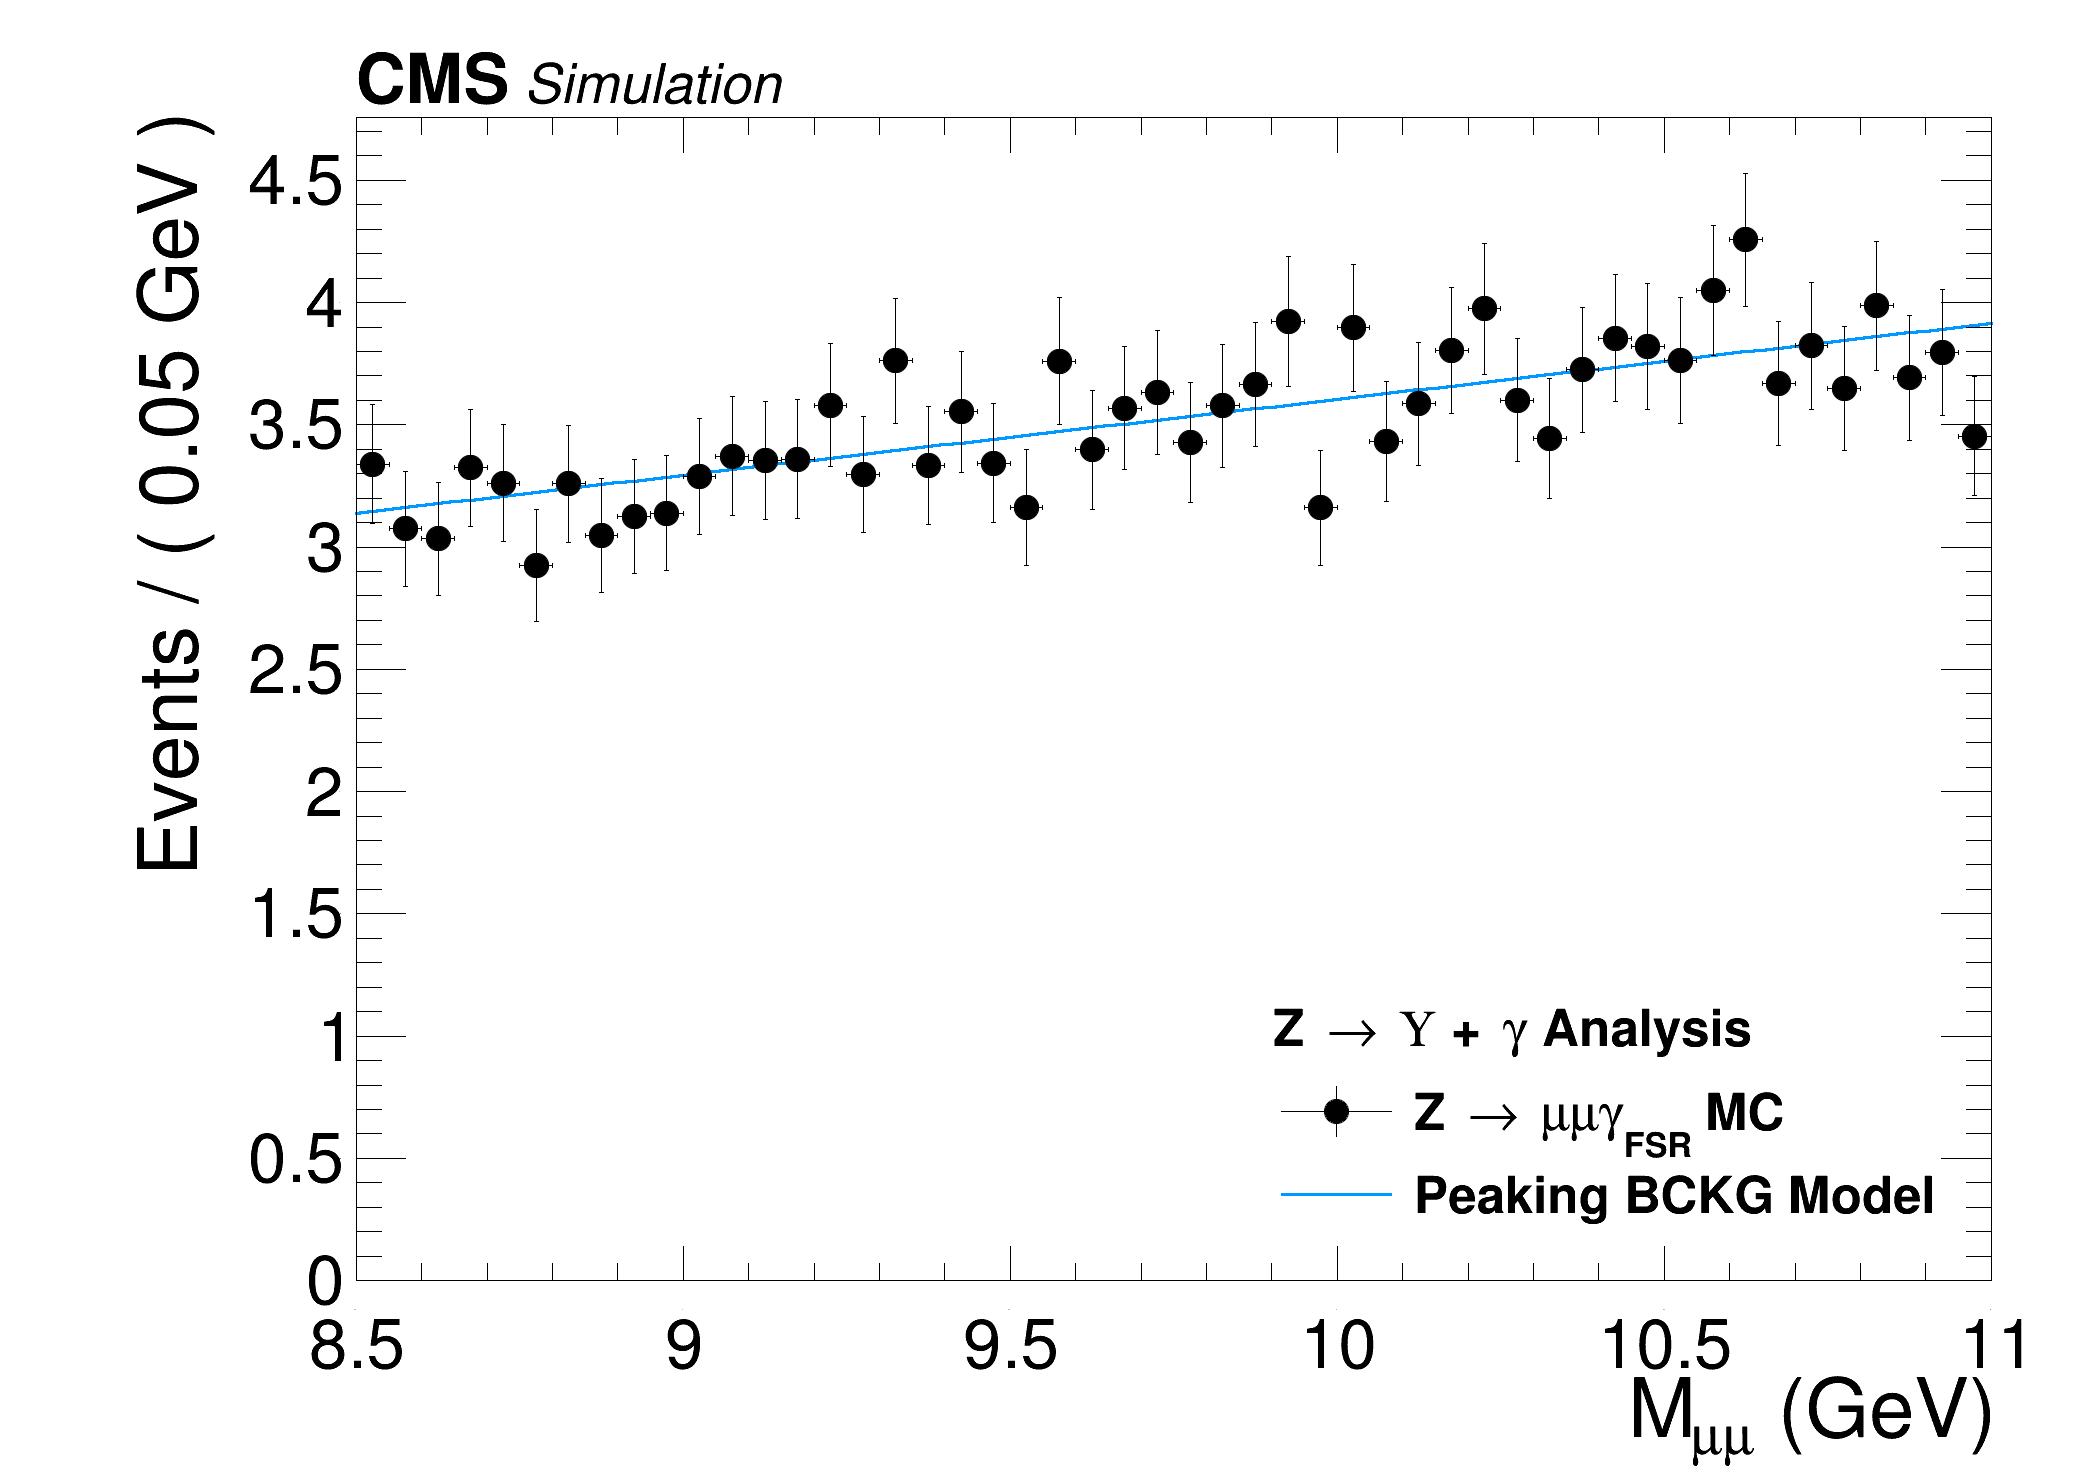
\includegraphics[width=0.45\textwidth]{figures_and_tables/fitPlotFiles2D/ZToUpsilonPhotonSignalAndBackgroundFit/mMuMNU_ZToUpsilon1SPhotonSignalAndBackgroundFit_PeakingBackground_Cat0}\hspace*{1.cm}
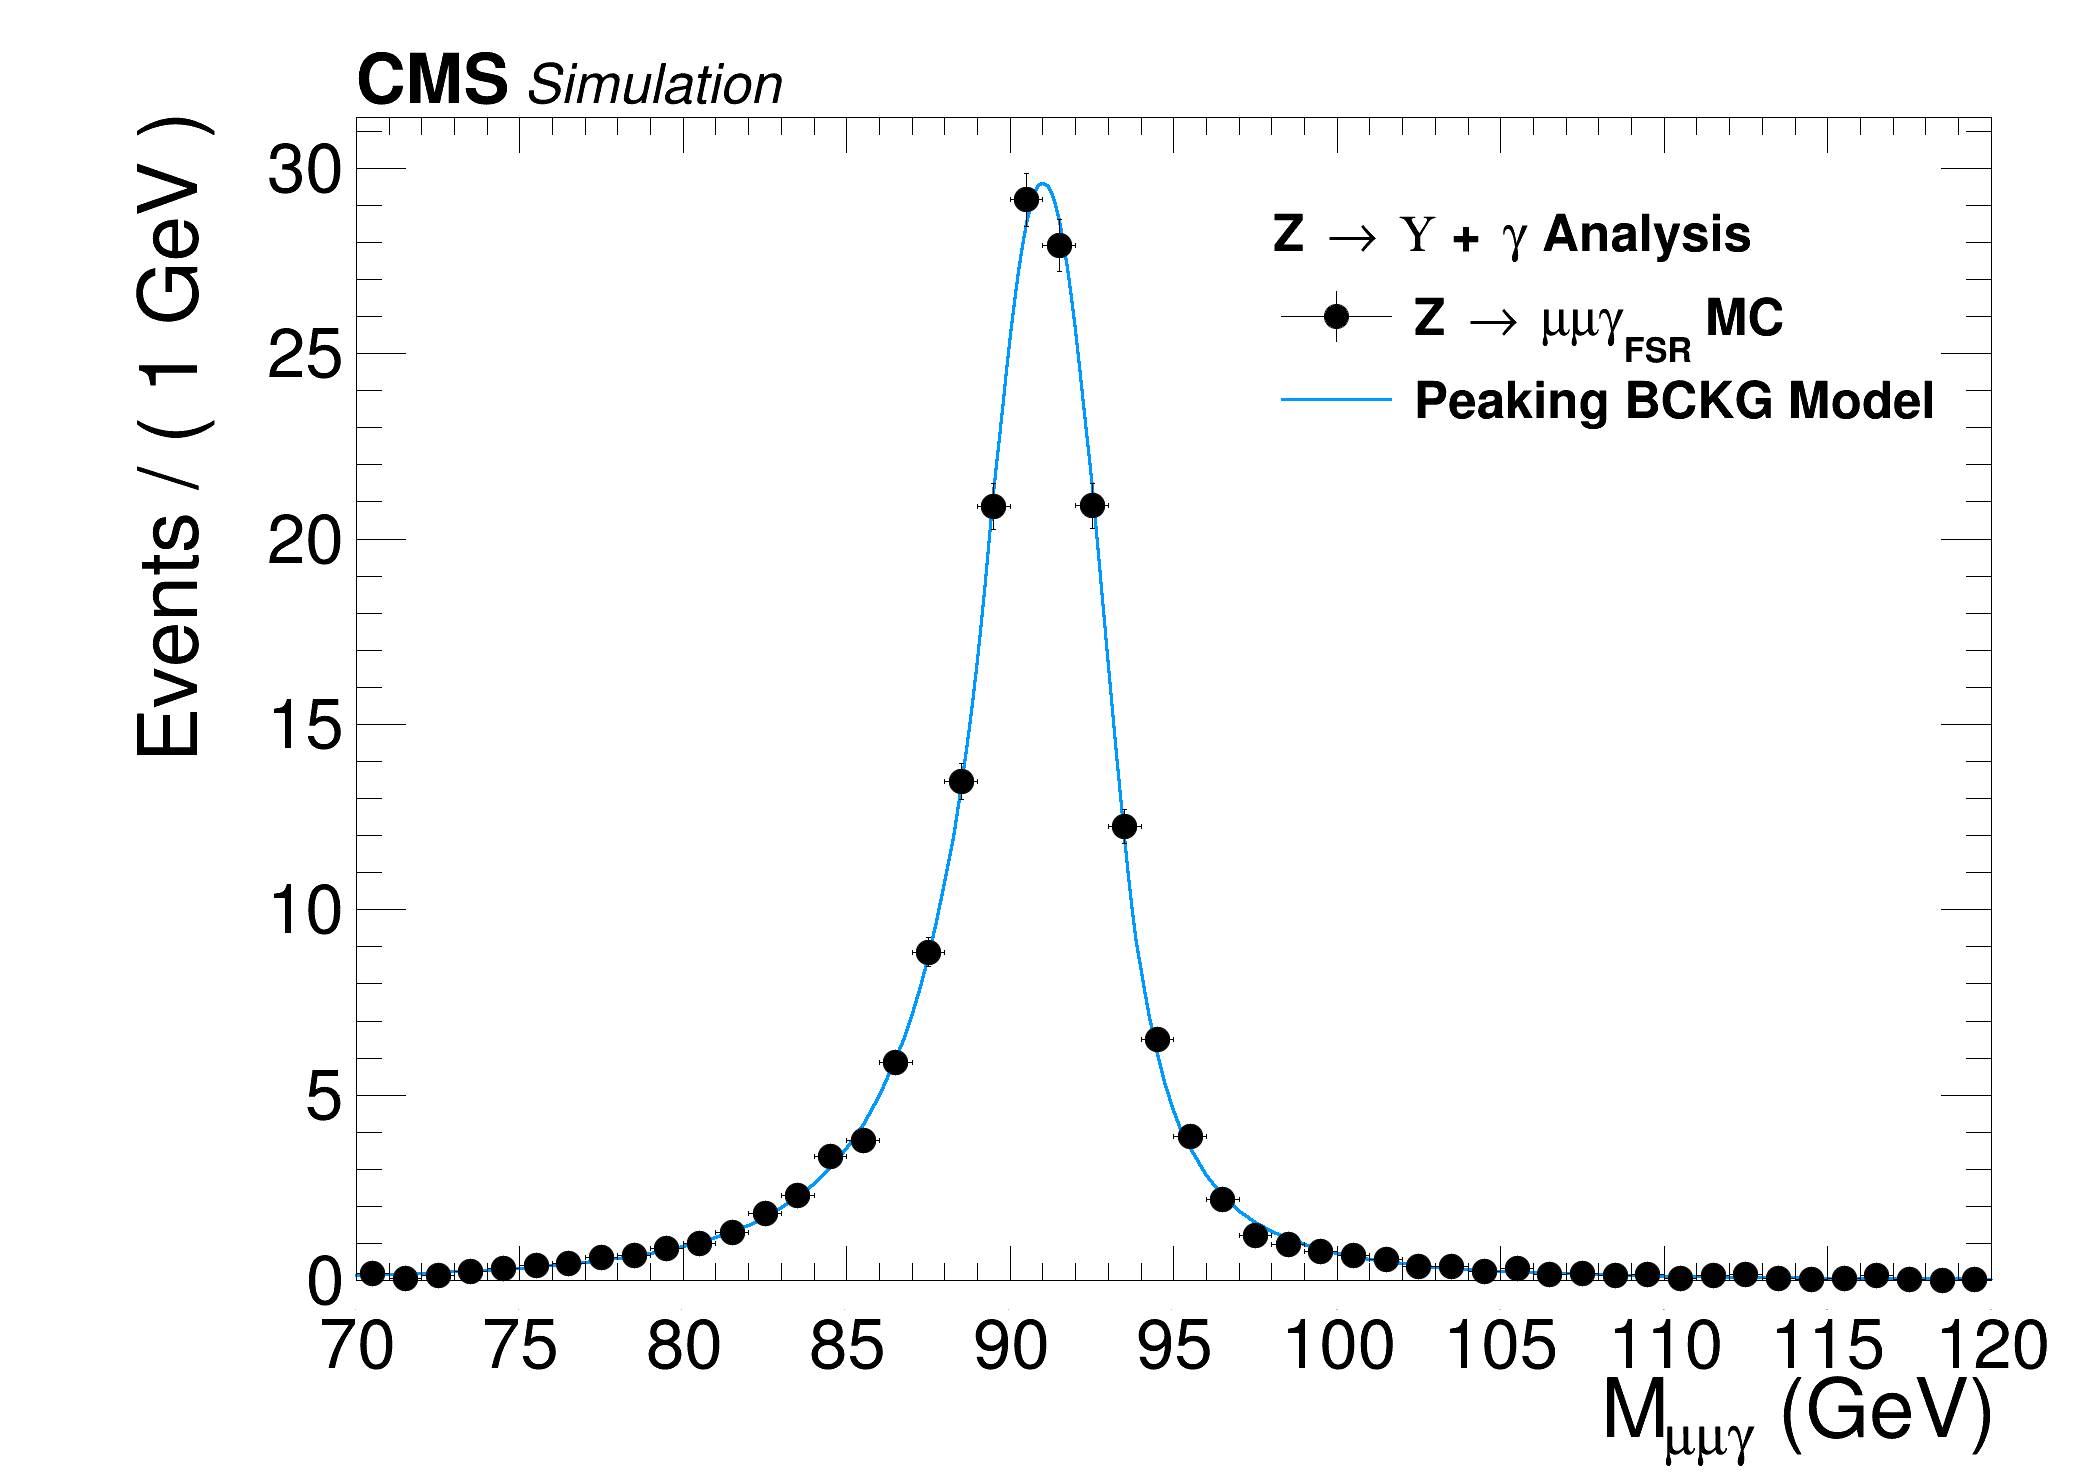
\includegraphics[width=0.45\textwidth]{figures_and_tables/fitPlotFiles2D/ZToUpsilonPhotonSignalAndBackgroundFit/mHZ_ZToUpsilon1SPhotonSignalAndBackgroundFit_PeakingBackground_Cat0}\hspace*{1.cm}

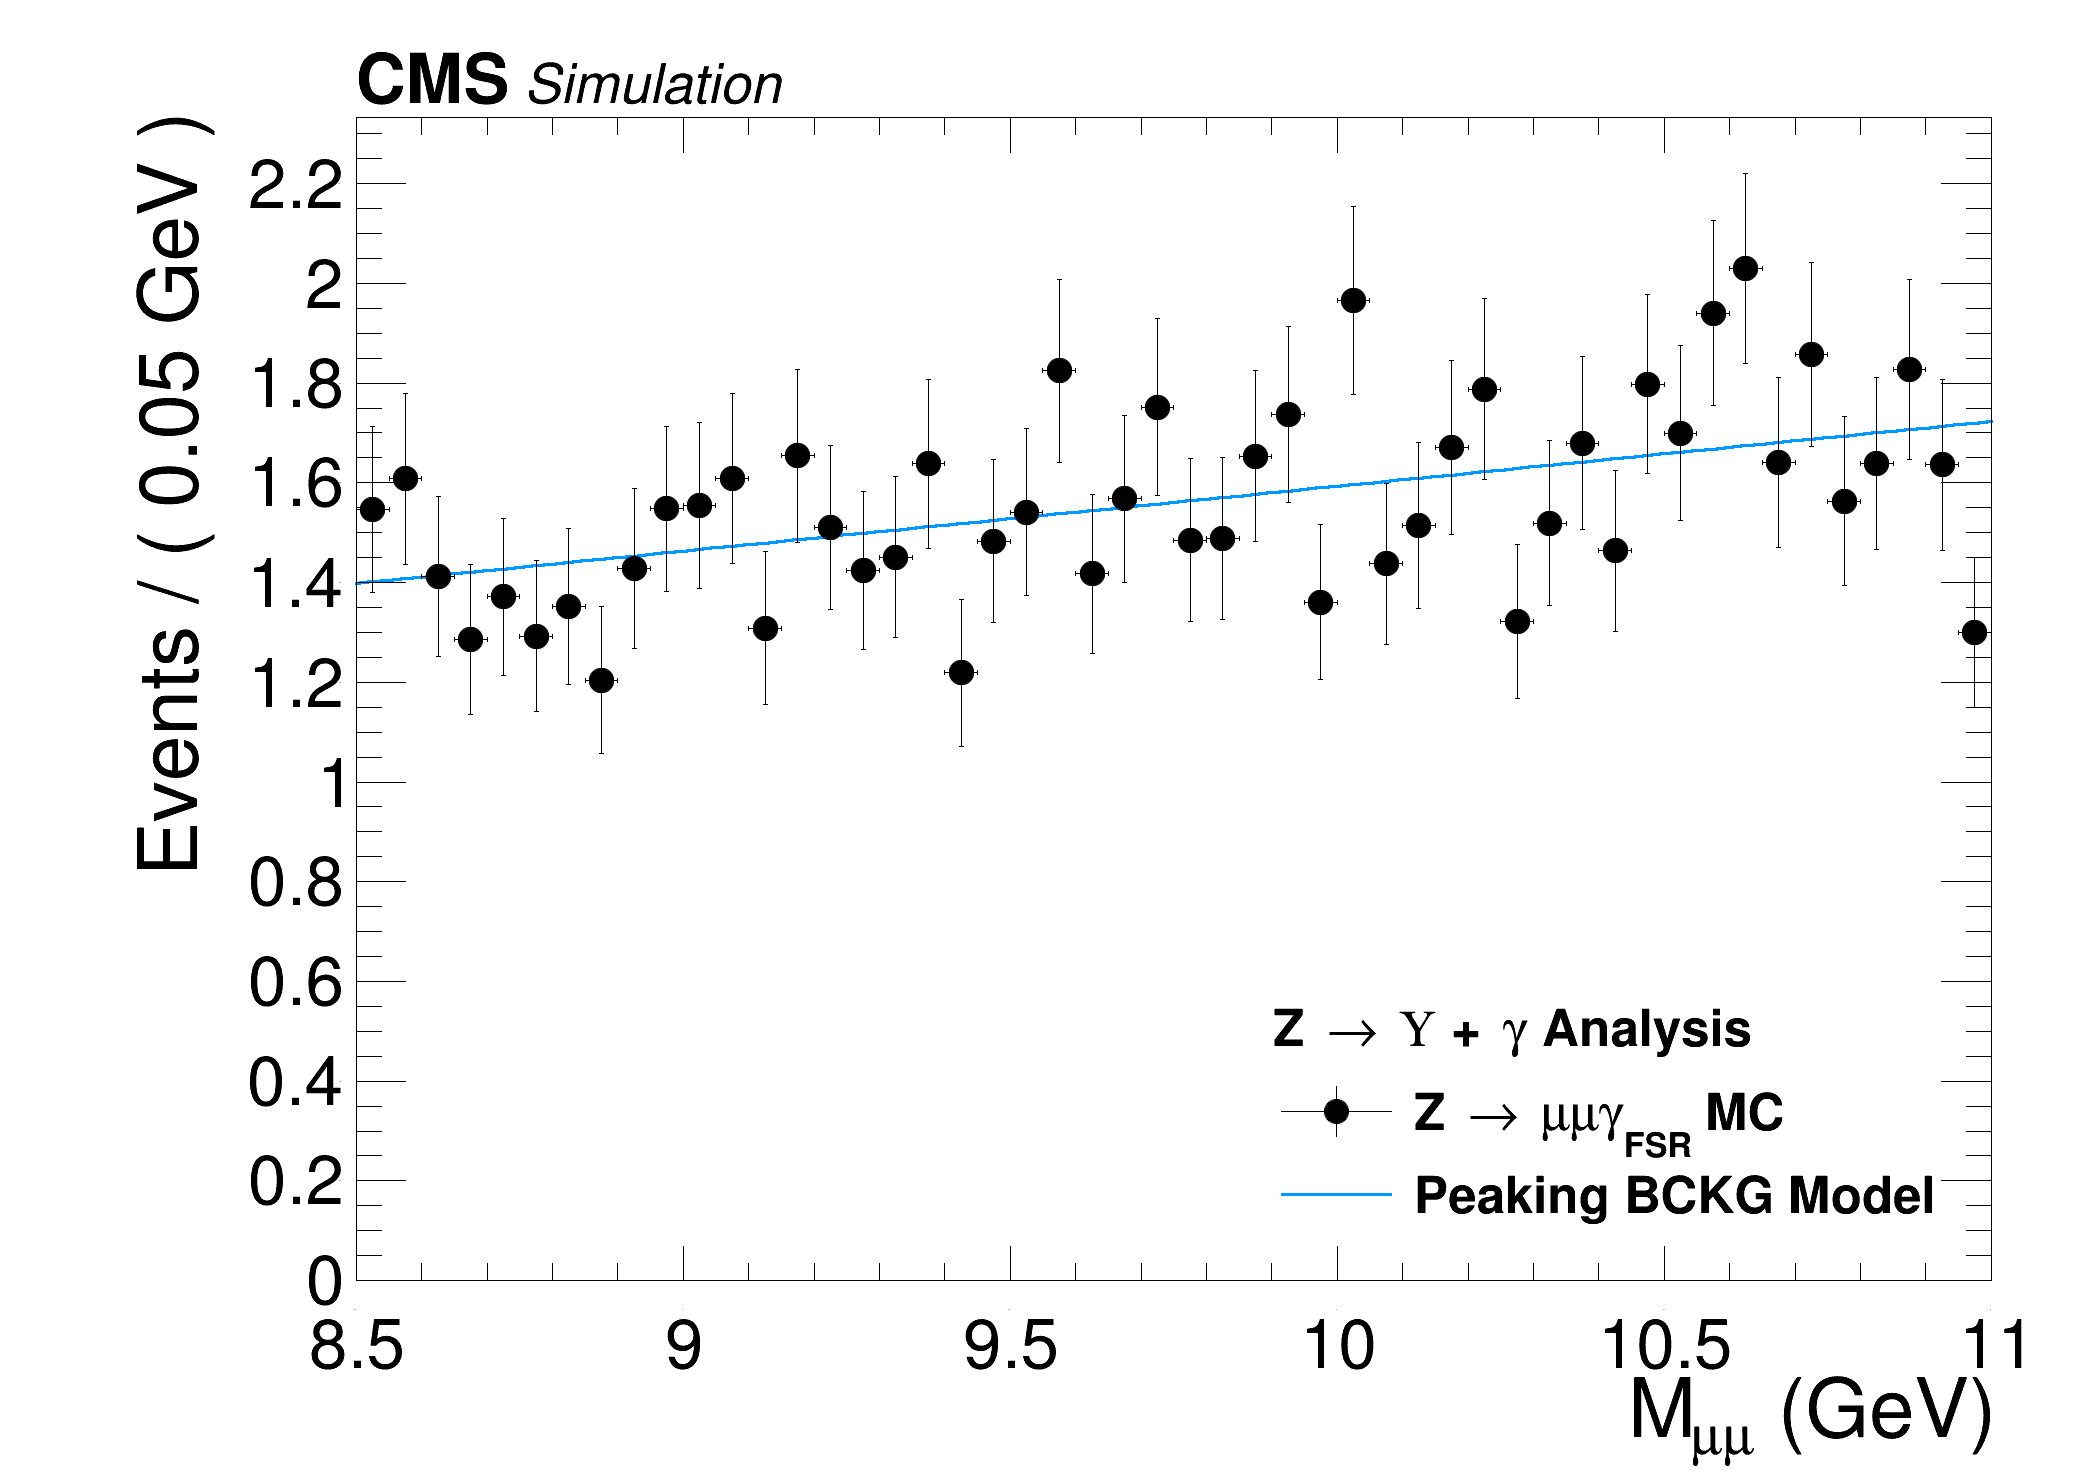
\includegraphics[width=0.45\textwidth]{figures_and_tables/fitPlotFiles2D/ZToUpsilonPhotonSignalAndBackgroundFit/mMuMNU_ZToUpsilon1SPhotonSignalAndBackgroundFit_PeakingBackground_Cat1}\hspace*{1.cm}
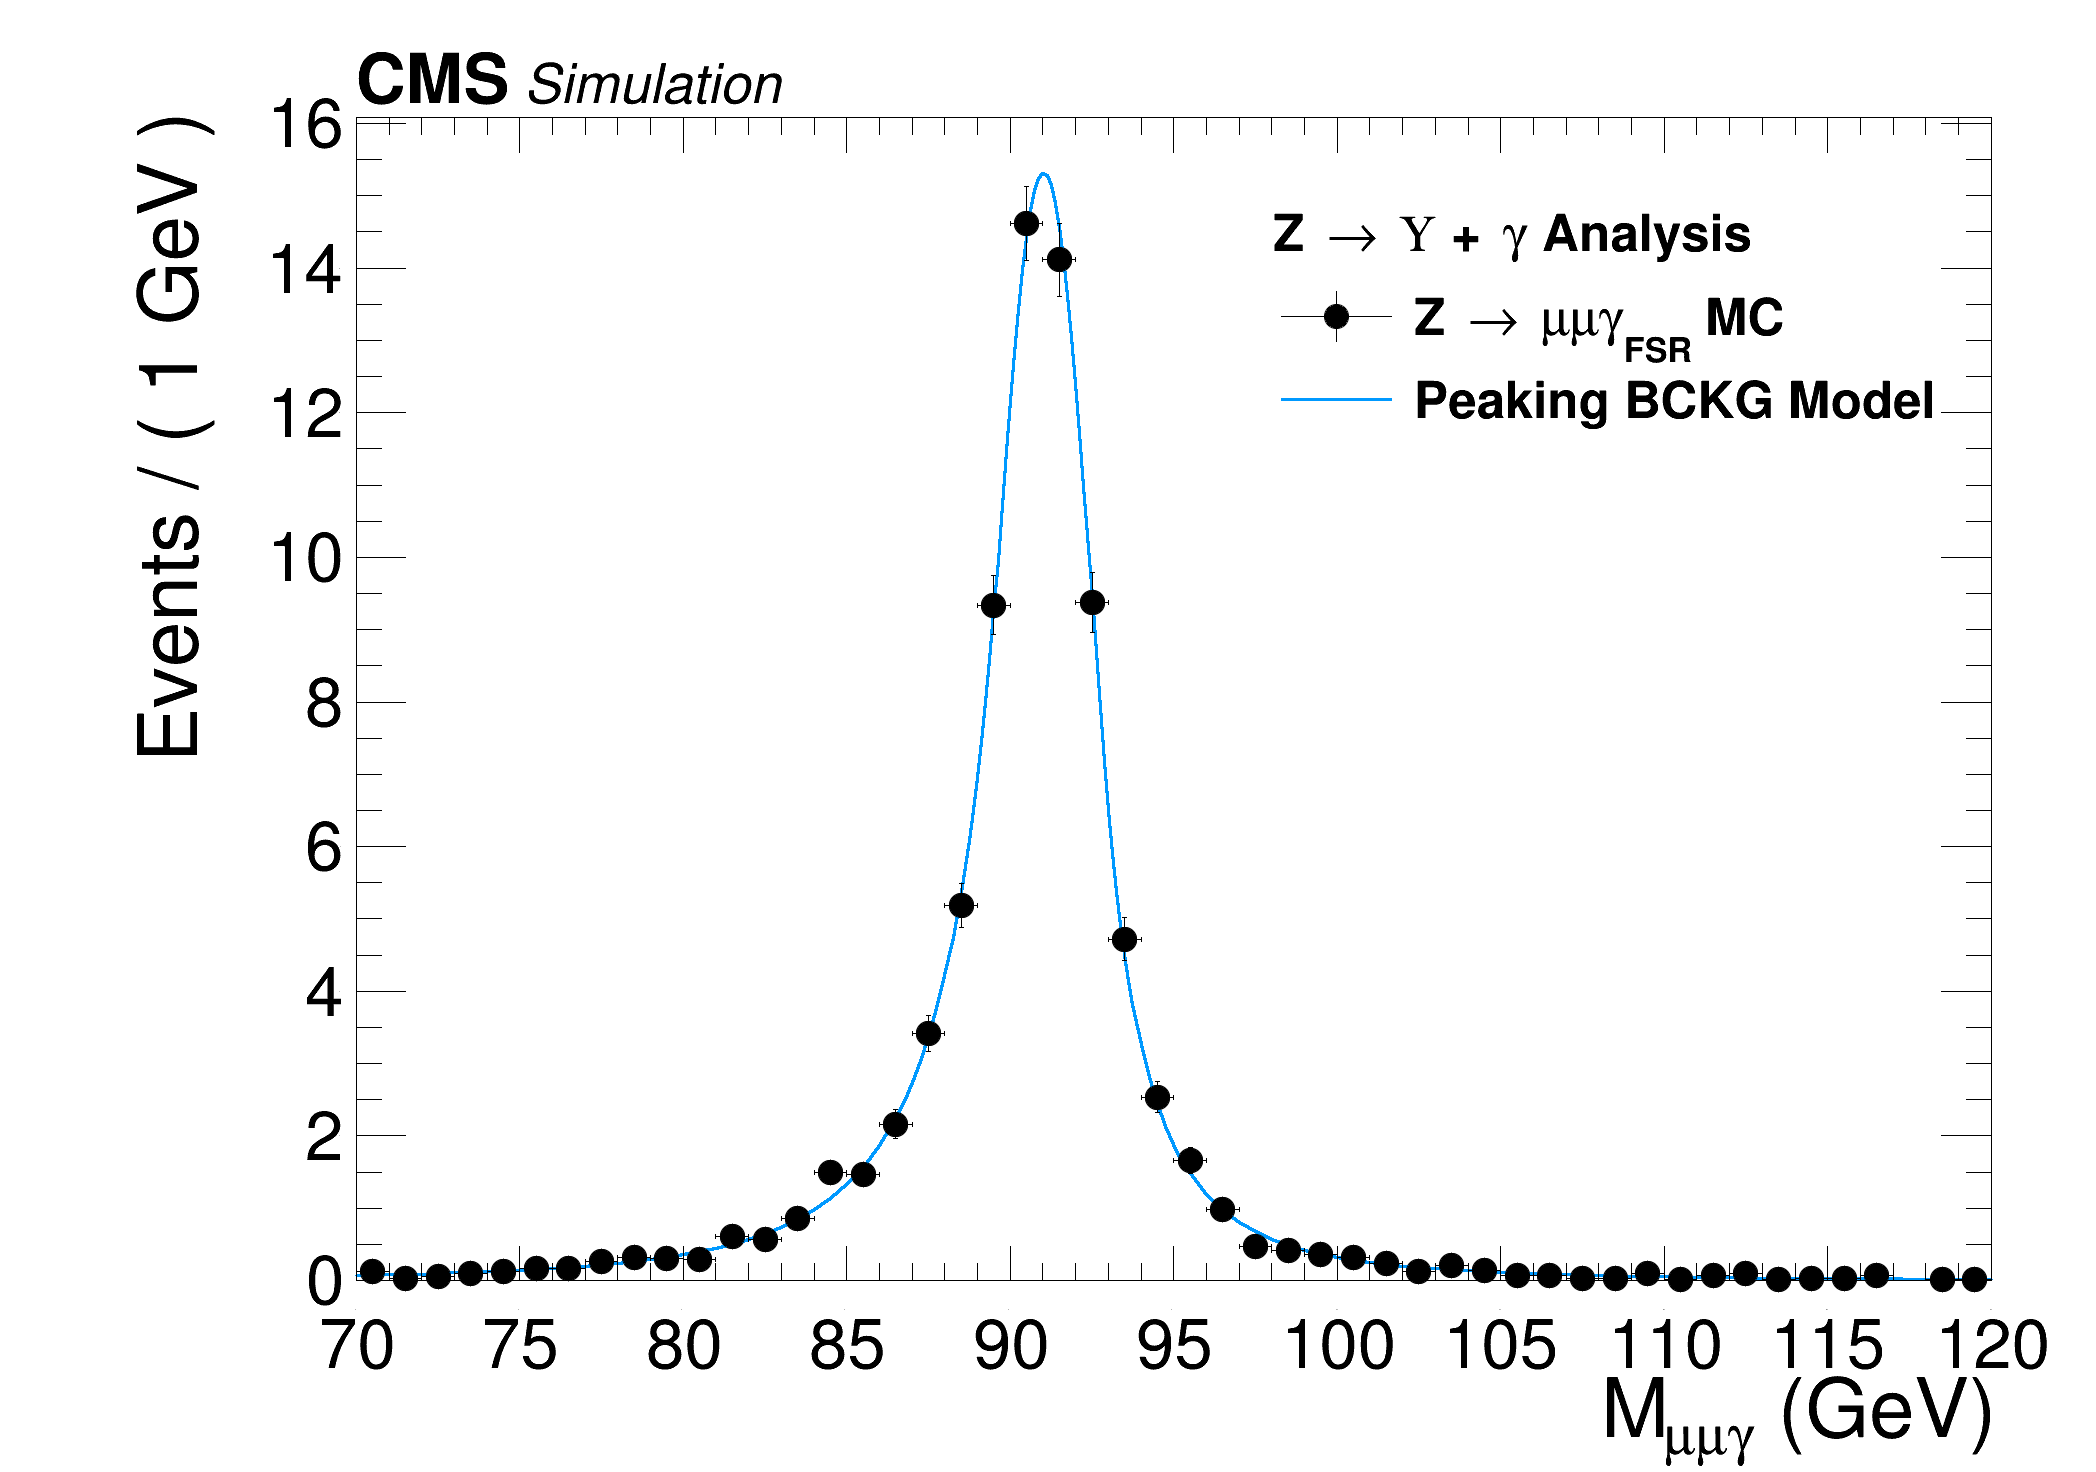
\includegraphics[width=0.45\textwidth]{figures_and_tables/fitPlotFiles2D/ZToUpsilonPhotonSignalAndBackgroundFit/mHZ_ZToUpsilon1SPhotonSignalAndBackgroundFit_PeakingBackground_Cat1}\hspace*{1.cm}

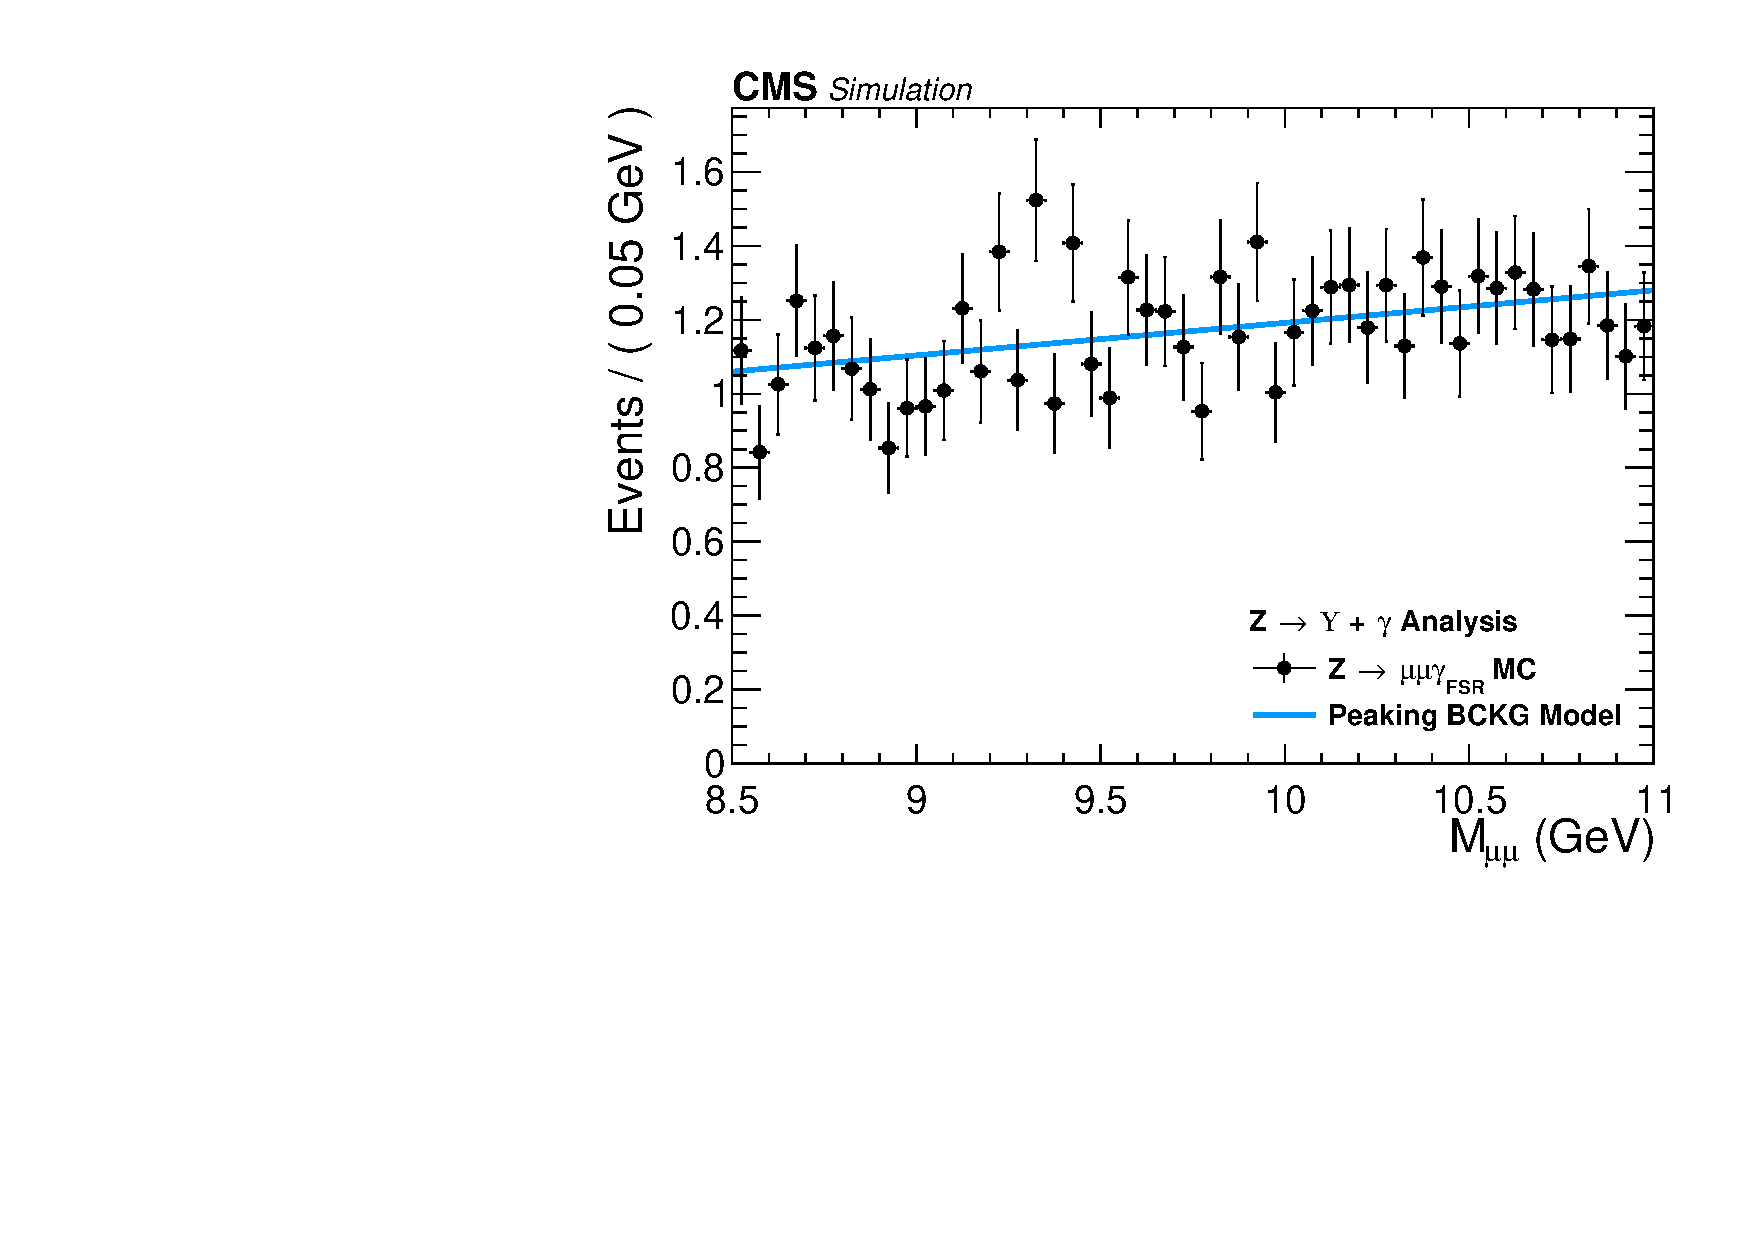
\includegraphics[width=0.45\textwidth]{figures_and_tables/fitPlotFiles2D/ZToUpsilonPhotonSignalAndBackgroundFit/mMuMNU_ZToUpsilon1SPhotonSignalAndBackgroundFit_PeakingBackground_Cat2}\hspace*{1.cm}
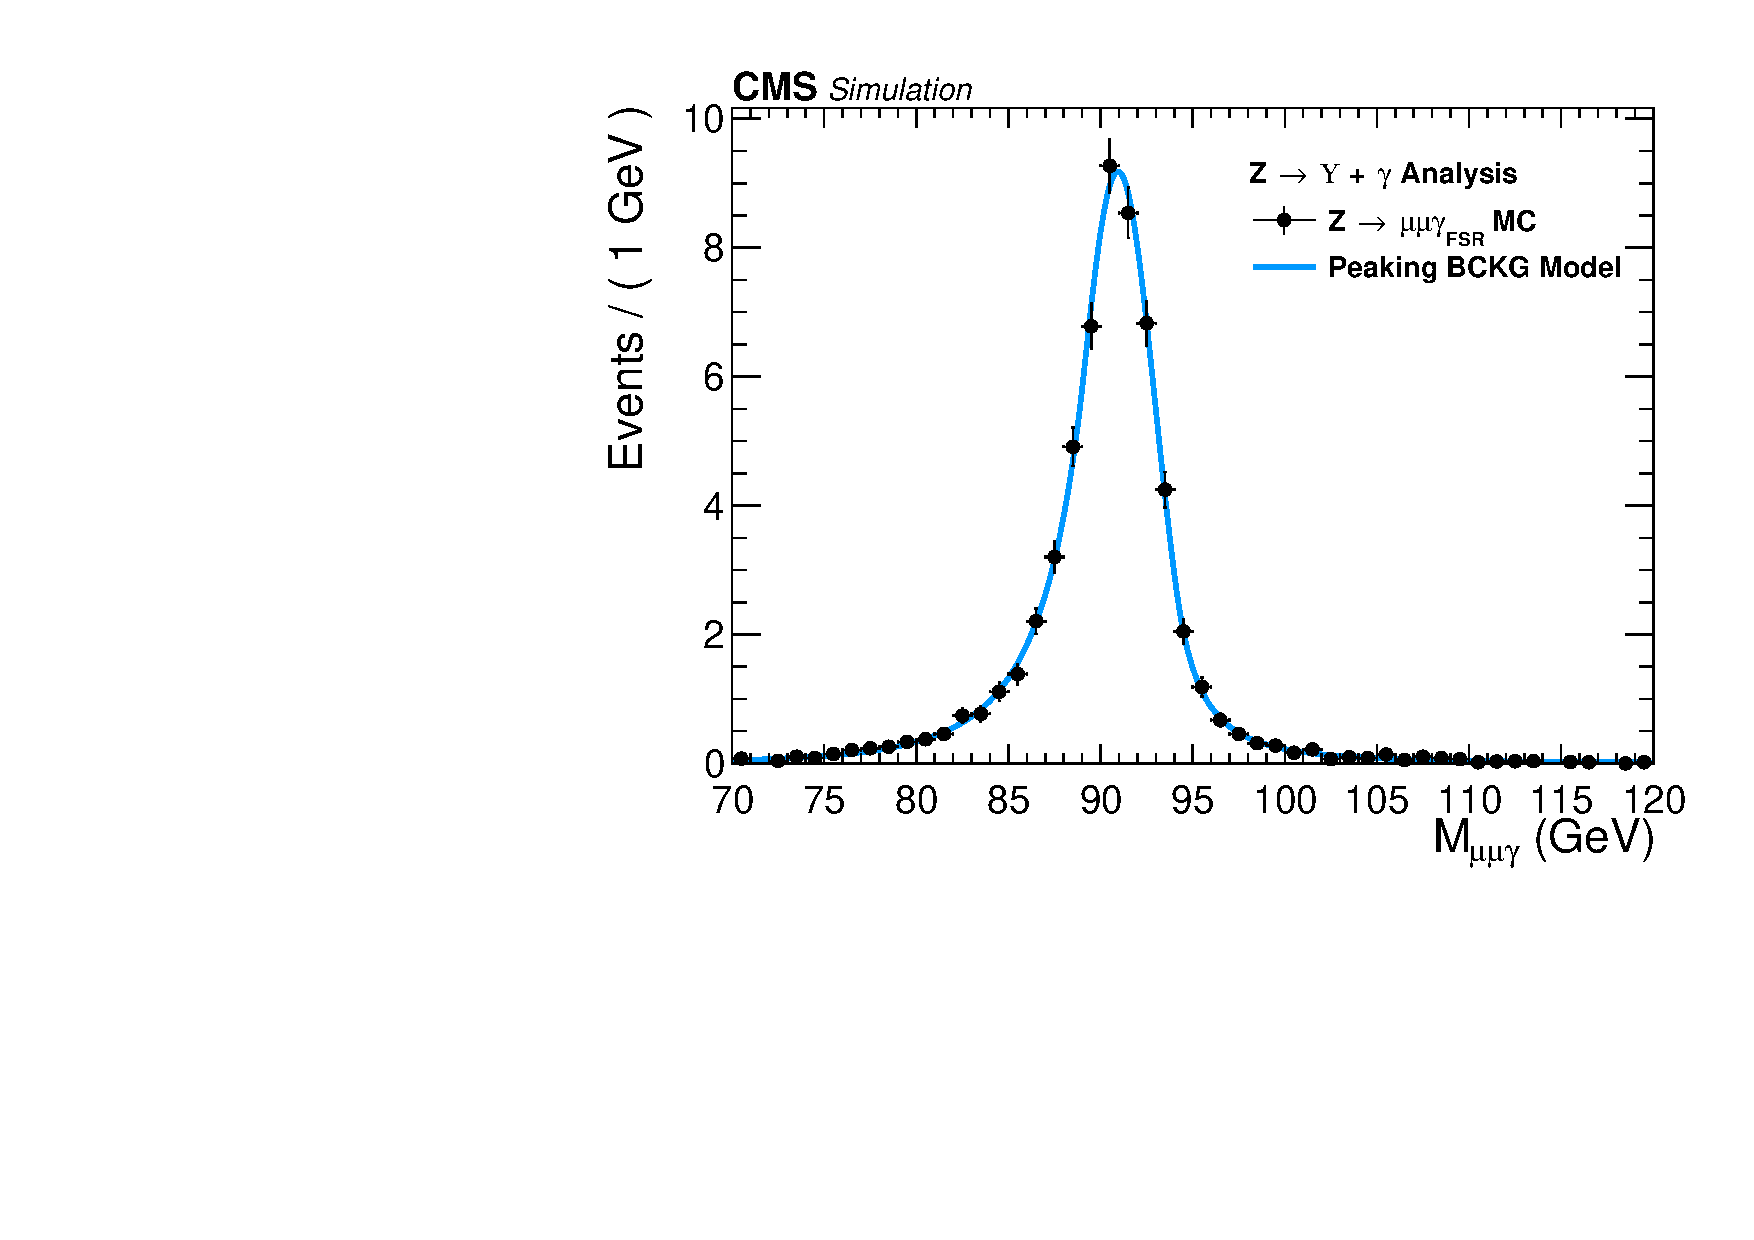
\includegraphics[width=0.45\textwidth]{figures_and_tables/fitPlotFiles2D/ZToUpsilonPhotonSignalAndBackgroundFit/mHZ_ZToUpsilon1SPhotonSignalAndBackgroundFit_PeakingBackground_Cat2}\hspace*{1.cm}

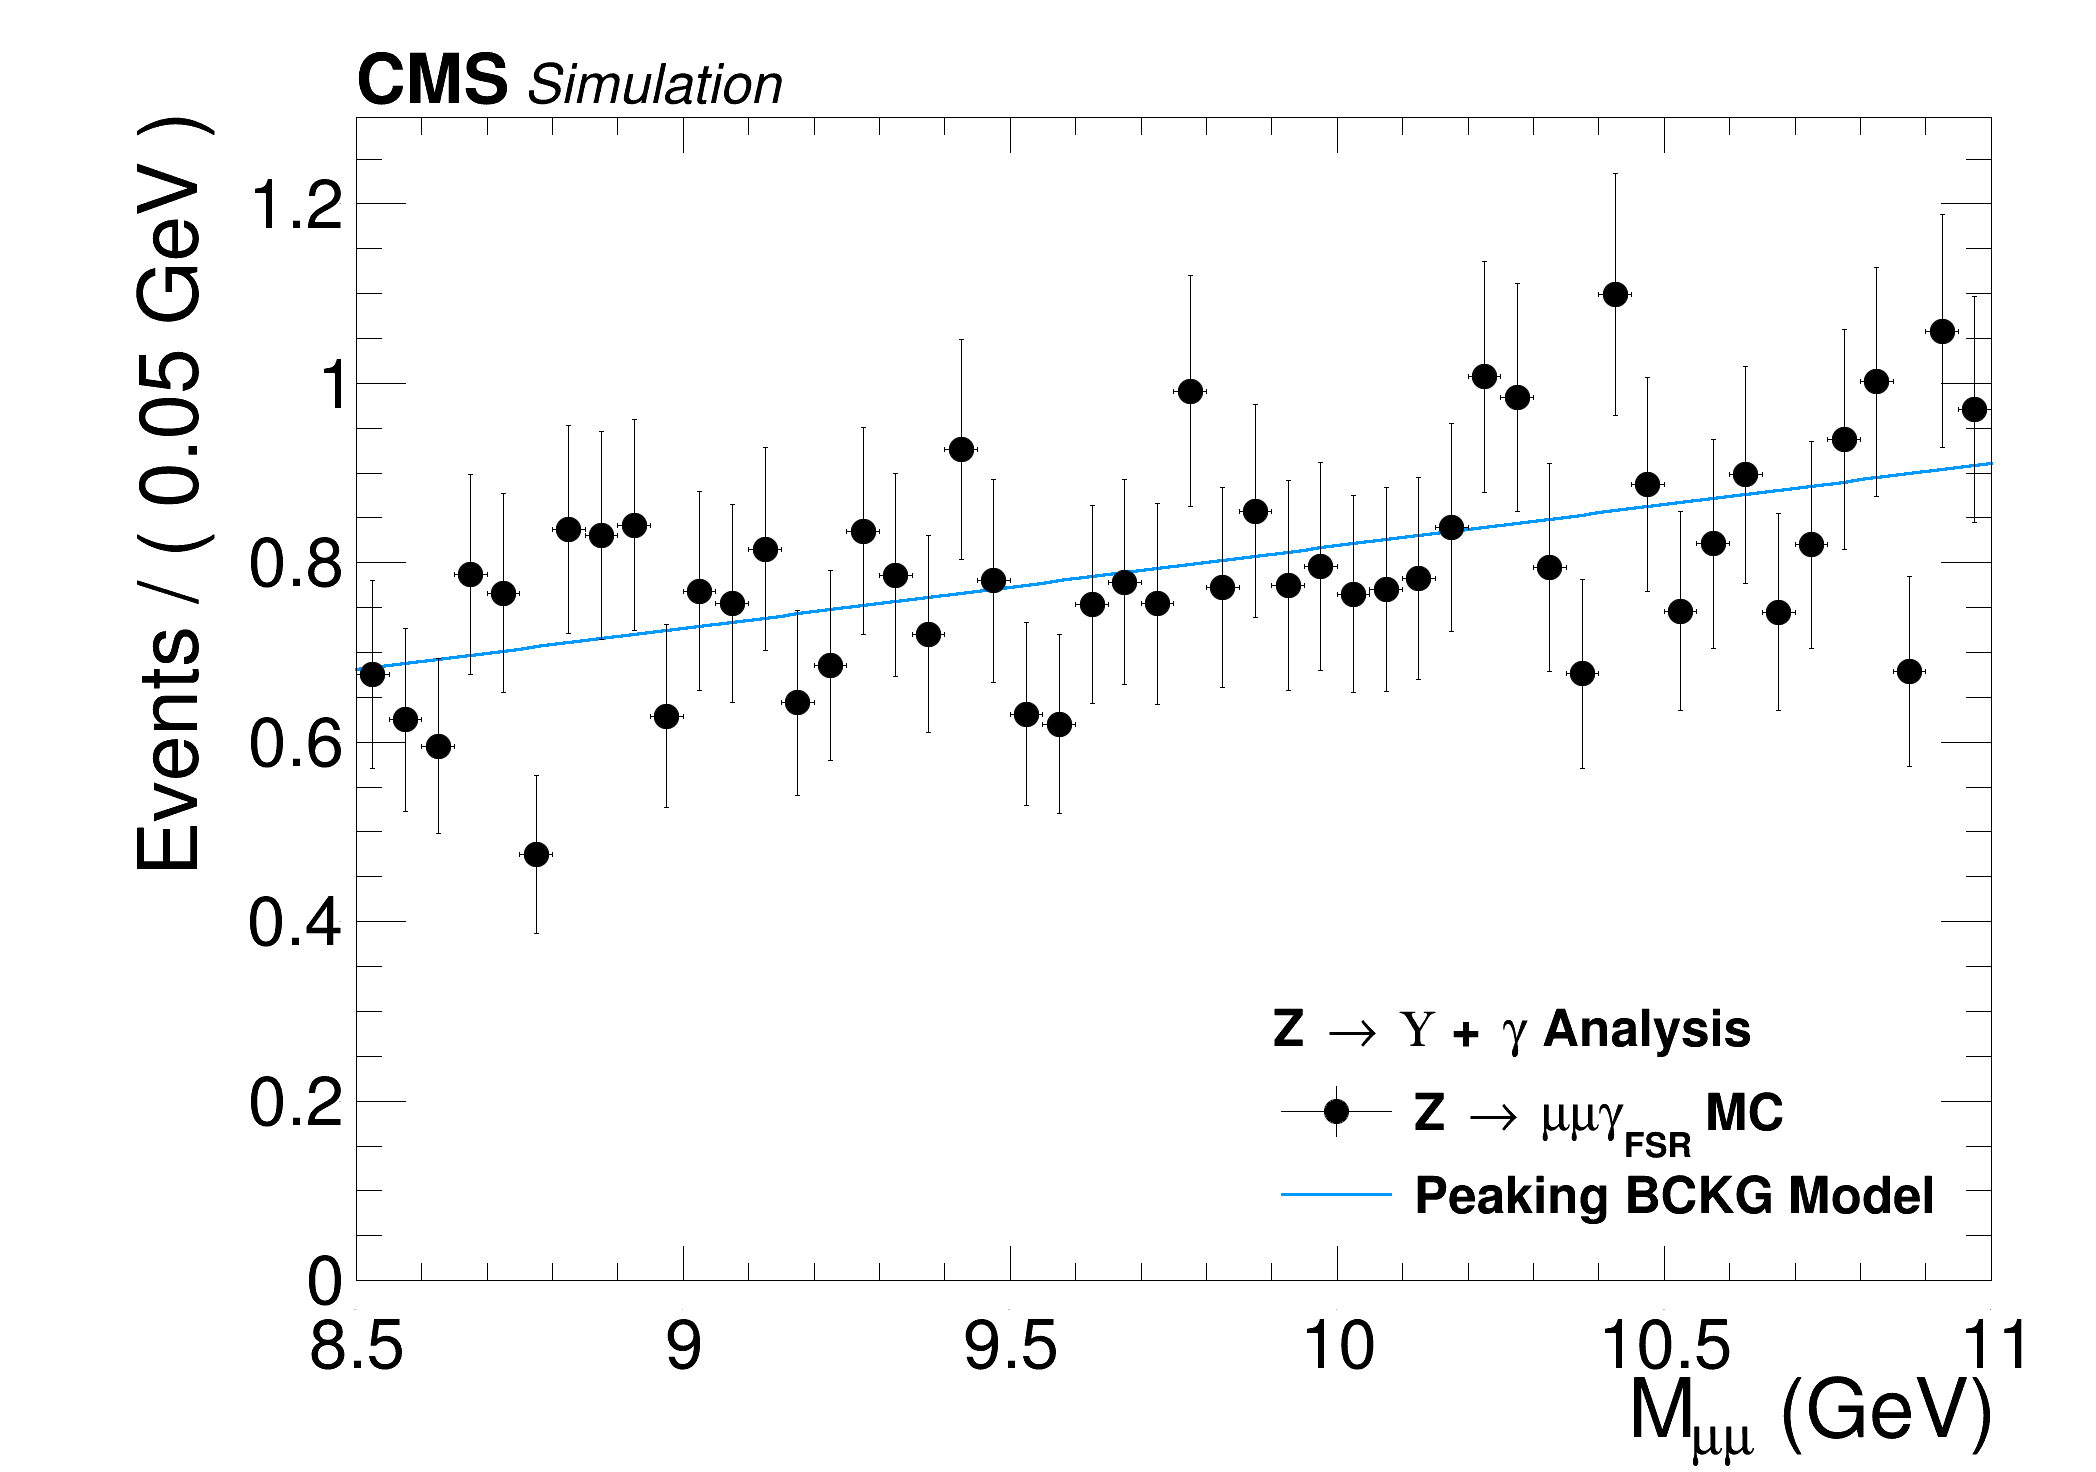
\includegraphics[width=0.45\textwidth]{figures_and_tables/fitPlotFiles2D/ZToUpsilonPhotonSignalAndBackgroundFit/mMuMNU_ZToUpsilon1SPhotonSignalAndBackgroundFit_PeakingBackground_Cat3}\hspace*{1.cm}
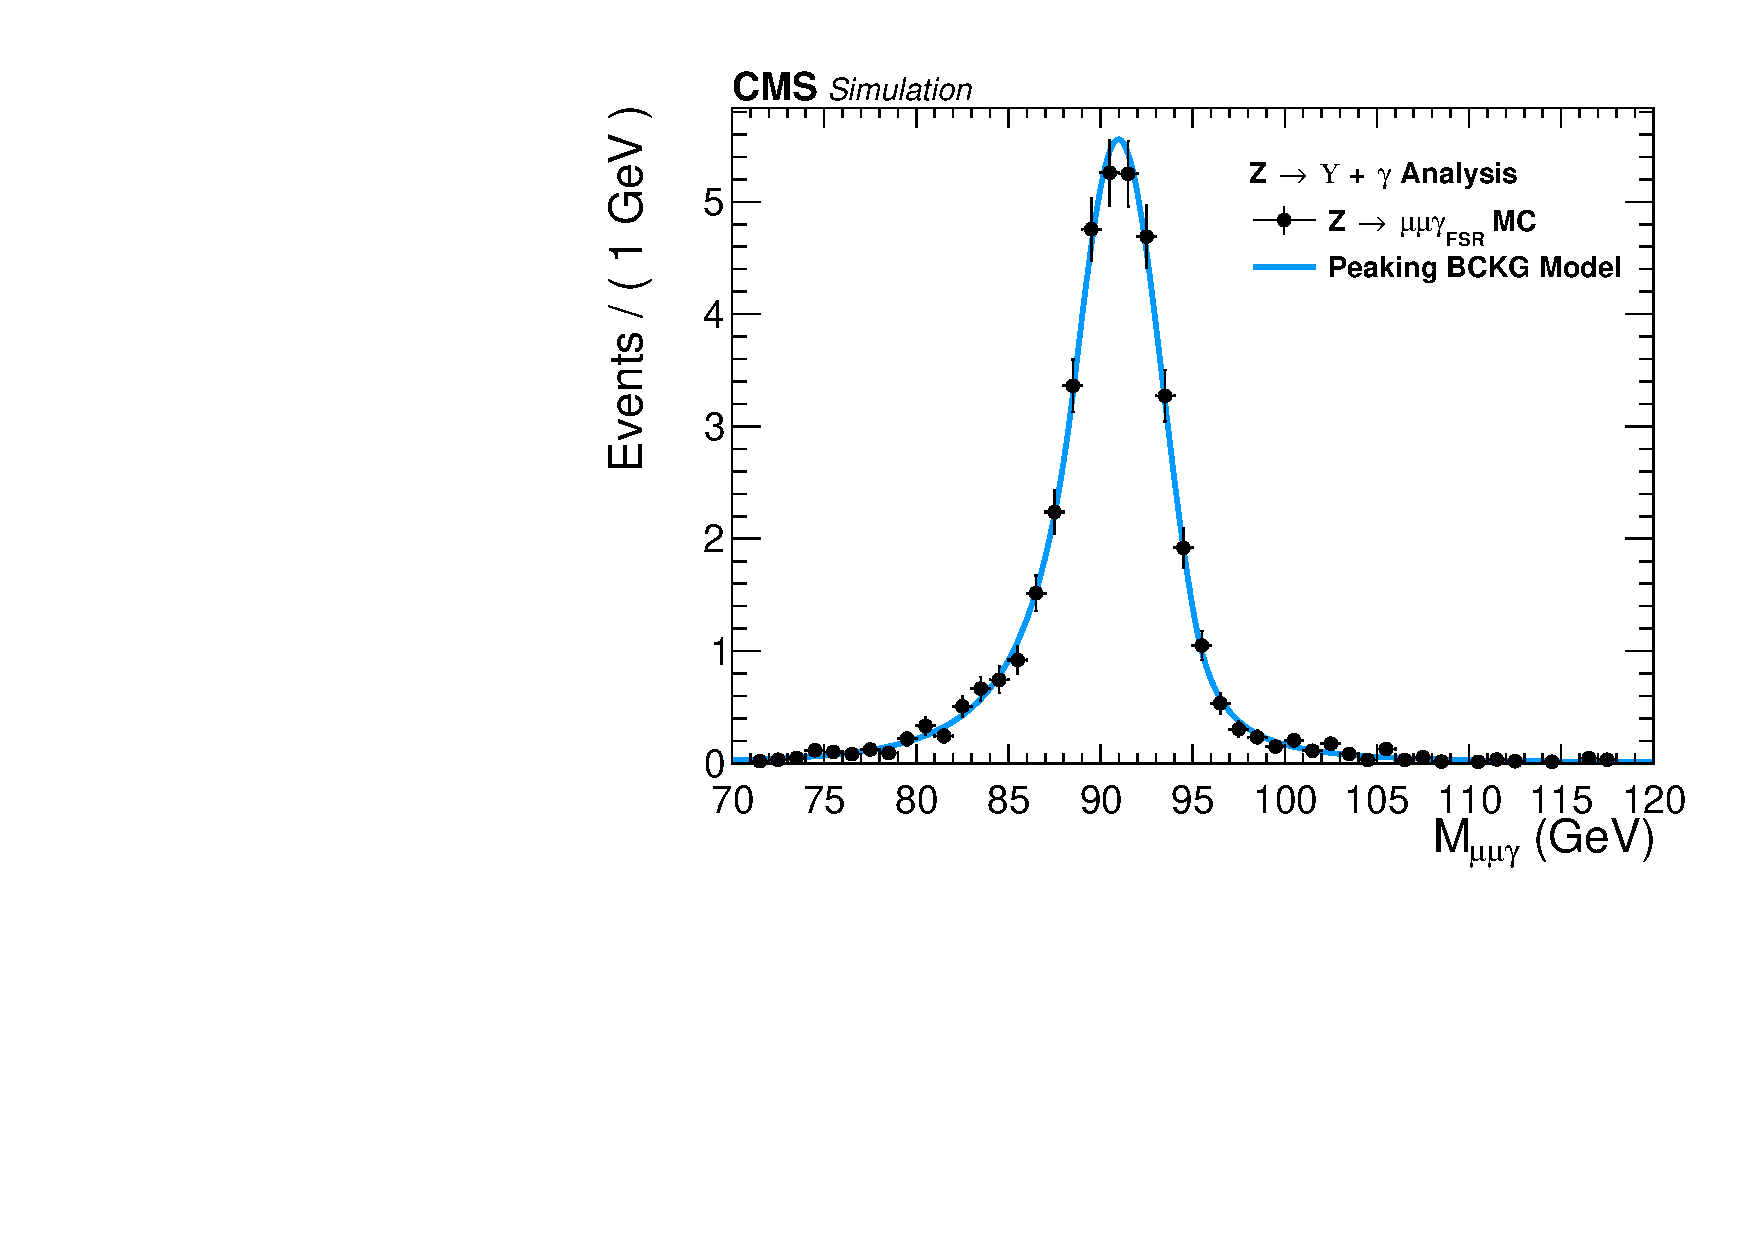
\includegraphics[width=0.45\textwidth]{figures_and_tables/fitPlotFiles2D/ZToUpsilonPhotonSignalAndBackgroundFit/mHZ_ZToUpsilon1SPhotonSignalAndBackgroundFit_PeakingBackground_Cat3}\hspace*{1.cm}


\end{center}\vspace*{-.5cm}
\caption{Resonant background for the $Z \rightarrow \Upsilon(1S,2S,3S) +\gamma$ analysis. $\mu\mu$ mass distribution (left) and $\mu\mu\gamma$ invariant mass distribution (right). From top to bottom categories: Inclusive, EB High R9, EB Low R9, EE.}
\label{fig:ZToUpsilon_PeakingBackground}
\end{figure}

For the three gaussian functions fits, which represent the three $\Upsilon$ states (1S, 2S and 3S) from the $\Upsilon$ Combinatorial background in the $m_{\mu\mu}$ component, we use a $\Upsilon$ control sample in order to extract the fit parameters, including the relative normalization between each $\Upsilon$ state. This sample is composed by dimuon candidates obtained from data, by selecting the events that passes the same trigger and dimuon selection of the nominal selection and with $p_{T}^{\mu\mu} > $ 35 GeV (this cut is done in order to keep this selected dimuon candidates compatibles with the $p_{T}^{\mu\mu}/M_{\mu\mu\gamma}$ cut applied in the nominal selection). No selection or cuts in the photon are required.


This control sample is fitted with a Chebychev 1\textsuperscript{st} order (linear polynomial) for the background support and 3 gaussian with the following constraints:

\begin{itemize}
  \item the mean of each state should be the ones in the PDG \cite{pdg_2020}, but allowed to shift by a float and common (the same for all states) value.
  \item the sigma should be based on the 1S fit of the MC. All other sigma should be the result of the 1S sigma times the state mass over the 1S mass ($\sigma_{2S,3S} = \frac{m_{2S,3S}}{m_{1S}} \sigma_{1S}$).
\end{itemize}

The idea behind this fit is that scale and resolution (mean and sigma, respectively, of the gaussians) over a sample without a photon selection should be the same as over a sample with photon selection, since these are detector-only dependent effects. The fact that we exclude the photon from this control sample, improves the statistics and gives a better measurement of these variables.

The fit of the $\Upsilon$ control sample is shown in figure \ref{fig:upsilon_control_Fit}.


\begin{figure}[!htbp]
\begin{center}

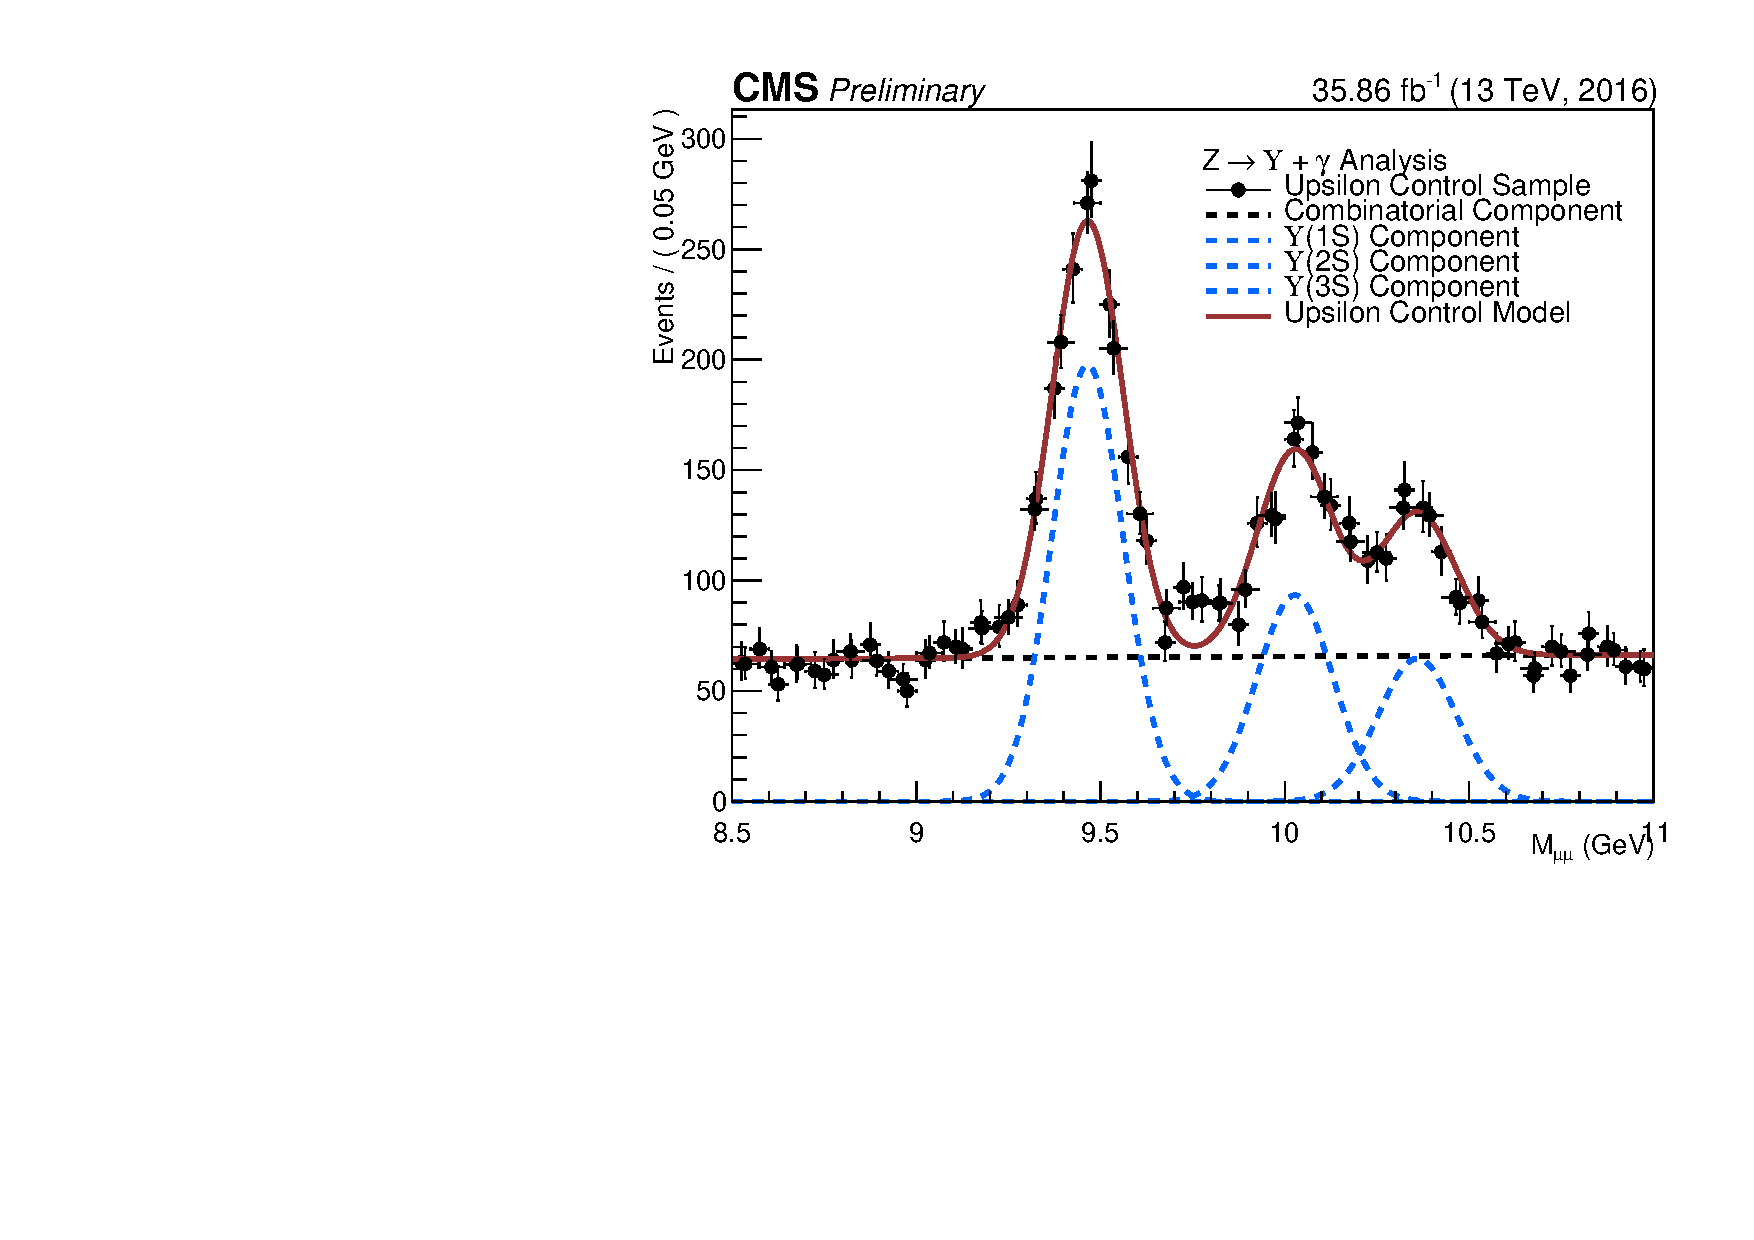
\includegraphics[width=0.60\textwidth]{figures_and_tables/fitPlotFiles2D/UpsilonControlSample/upsilonControlSample_ZToUpsilonPhoton_Cat0}

\end{center}\vspace*{-.5cm}

\caption{$\Upsilon$ control sample fit with Chebychev 1\textsuperscript{st} order for the background support and 3 gaussian for the three $\Upsilon(1S,2S,3S)$ peaks.}
\label{fig:upsilon_control_Fit}
\end{figure}


% Once determined, the fit parameters above are fixed and used to compose the 2-Dimensional \textit{pdf} The $m_{\mu\mu}$ component of the full combinatorial background is derived fully from the data fit (described below). In the same sense, the $m_{\mu\mu\gamma}$ component of the full combinatorial and the $\Upsilon$ Combinatorial backgrounds are also fully derived from the data, but following a much complex procedure: a composition with the \textit{pdf} components described above, plus a F-Test within a Discrete Profiling (or "Envelope Method").


Once determined, the fit parameters are fixed, they are used to compose the 2-Dimensional \textit{pdf}. The $m_{\mu\mu}$ component of the full combinatorial background is derived fully from the data fit (described below). In the same sense, the $m_{\mu\mu\gamma}$ component of the full combinatorial and the $\Upsilon(nS)$ Combinatorial backgrounds are also fully derived from the data, but following a more complex procedure: a composition with the \textit{pdf} components described above, plus a statistical test, to avoid overfitting within a Discrete Profiling (or "Envelope Method"), as described in~\cite{DiscreteProfilingMethod} and also implemented in~\cite{higgs_gammagamma_PAPPER}. 

The statistical test consists of, for each category, different orders of a set of polynomial \textit{pdfs} families are tested: a sums of exponentials, sum of polynomials (in the Bernstein basis), a Laurent series and a sums of power-law functions. 


\begin{itemize}
\item Sums of exponentials: $$ f_{N}(x)= \sum^{N}_{i=1} p_{2i} e^{p_{2i+1} x} ,$$
\item Sums of polynomials (in the Bernstein basis): $$ f_{N}(x) = \sum^{N}_{i=0} p_{i} b_{(i,N)}, \text{ where } b_{(i,N)}:= \begin{pmatrix} N \\ i \end{pmatrix} x^i (1-x)^{N-i} ,$$
\item Laurent series: $$ f_{N}(x)= \sum^{N}_{i=1} p_{i} x^{-4 + \sum^{i}_{j=1} (-1)^{j} (j-1)},$$
\item Sums of power-law functions: $$ f_{N}(x)= \sum^{N}_{i=1} p_{2i} x^{-p_{2i+1}},$$
\end{itemize}
where for all $k$, the $p_k$ are a set of floating parameters in the fit.

Twice difference in the negative log-likelihood ($NLL$) between the $N^{th}$ and the $(N+1)^{th}$ order of the same polynomial ($\Delta NLL = 2 \times (NLL_{N} - NLL_{N+1})$) is expected to follow a $\chi^2$ distribution with $M$ degrees of freedom, where $M$ is the increase in degrees of freedom when going from $N^{th}$ to $(N+1)^{th}$. This can be shown with the help of the Wilks' theorem~\cite{wilks1938}. 
% In summary, a likelihood ratio test in the form of $\Lambda = \mathcal{L(\theta_{null})}/\mathcal{L(\theta_{alternative})}$, between the null hypotheses and an alternative one, , 

% \begin{equation}
% \label{eqn:wilks}
% -2log(\Lambda) \sim \chi^2_M,
% \end{equation}
% where $\Lambda$ is a likelihood ratio test in the form of $\Lambda = \mathcal{L(\theta_{null})}/\mathcal{L(\theta_{alternative})}$, between the null hypotheses and an alternative one.

Starting from the lowest order possible, the best choice of order, for each family, is determined when a increase in the order of the polynomial, does not brings a significant improvement in the quality of the fit. Since a model with more fit parameters (higher order polynomials) will always perform, if not the same, better than a simpler one, an optimal choice of the polynomial order, will be the one right before the model becomes too flexible for the data.

Consider a $p$-value defined as: 

\begin{equation}
\label{eqn:p-value_f_test}
\begin{split}
 p\text{-value} & = \int^{\infty}_{\Delta NLL} \chi^2_M(\Delta) \text{ } d\Delta\\
& = P(\chi^2_M > \Delta NLL)  ,
\end{split}
\end{equation}

In the same spirit as the Wilks' theorem, this is the $p$-value for a likelihood ratio test between a null hypotheses and an alternative model, where the null hypotheses is the $N^{th}$ order and $(N+1)^{th}$ order is the alternative one.

\begin{equation}
\label{eqn:likehood_ratio}
\begin{split}
 \Delta NLL & = 2 \times (NLL_{N} - NLL_{N+1}) \\
  & = -2 \times log(\frac{\mathcal{L}_N}{\mathcal{L}_{N+1}}),
\end{split}
\end{equation}
where $\mathcal{L}_N$ is the likelihood for the $N^{th}$ polynomial order.

The alternative will present a statistically significant improvement, with respect to the null hypotheses, if the $p$-value is smaller than 0.05, since the probability of obtaining, by chance, considering the null hypotheses is true, a even higher $\Delta NLL$ is less than 5\%. This will give support to chose $(N+1)^{th}$ over $N^{th}$.

If the $p$-value is greater than 0.05 a higher order is not supported, since the probability of obtaining a $\Delta NLL$ greater than the one observed is statistically significant (more than 5\%). A higher $\Delta NLL$ means that another data sample, collected and analyzed with strictly the same conditions, would have a probability of more than 5\% of giving a better fit improvement than the one observed, again assuming that the null hypotheses is true. This is an indication of overfitting, since the improvements are likely to come from just statistical fluctuations. When testing the $(N+1)^{th}$ order and this condition is reached, the optimal order should be the $N^{th}$.

At first, before any fit to data, the 2-Dimensional model is composed by the five components, as described in Table \ref{tab:BckgModeling_Z} (in which the $m_{\mu\mu\gamma}$ modeling for the Full Combinatorial Background and the $\Upsilon$ combinatorial are shared), then, the statistical test described before is ran for each family. It is important to stress that before the statistical test all the other fitting parameters have been fixed. This leaves only the normalizations of the model components and the polynomial coefficients free to float.

Once the optimal order for each \textit{pdf} family is obtained, the composed \textit{pdf} with each choice from statistical test is saved in the same model, providing a discrete variable that indexes the different polynomial \textit{pdf} families. This method is called Discrete Profiling (or \textit{"Envelope Method"}) and it allows the analysis algorithm to treat the choice of the \textit{pdf} as a systematics and incorporate its effect in the extracted upper limits. This model, with different choices of polynomial families is called envelope.

The implementation, used in the analysis, of the statistical test and the Discrete Profiling is based on the same algorithm used by the $H \rightarrow \gamma\gamma$ Run II analysis. An extensive documentation on these methods can be found in $H \rightarrow \gamma\gamma$ analysis note and physics analysis summary \cite{higgs_gammagamma_AN, higgs_gammagamma_PAS} and in the specific reference of the Discrete Profiling \cite{DiscreteProfilingMethod}. The figures \ref{fig:ZToUpsilon_mMuMU_Projection} and \ref{fig:ZToUpsilon_mHZ_Projection} show the projection for the $\mu\mu$ and $\mu\mu\gamma$ distribution after the statistical test.

% Z To Upsilon - mMuMU Projection
\begin{figure}[!htbp]
\begin{center}
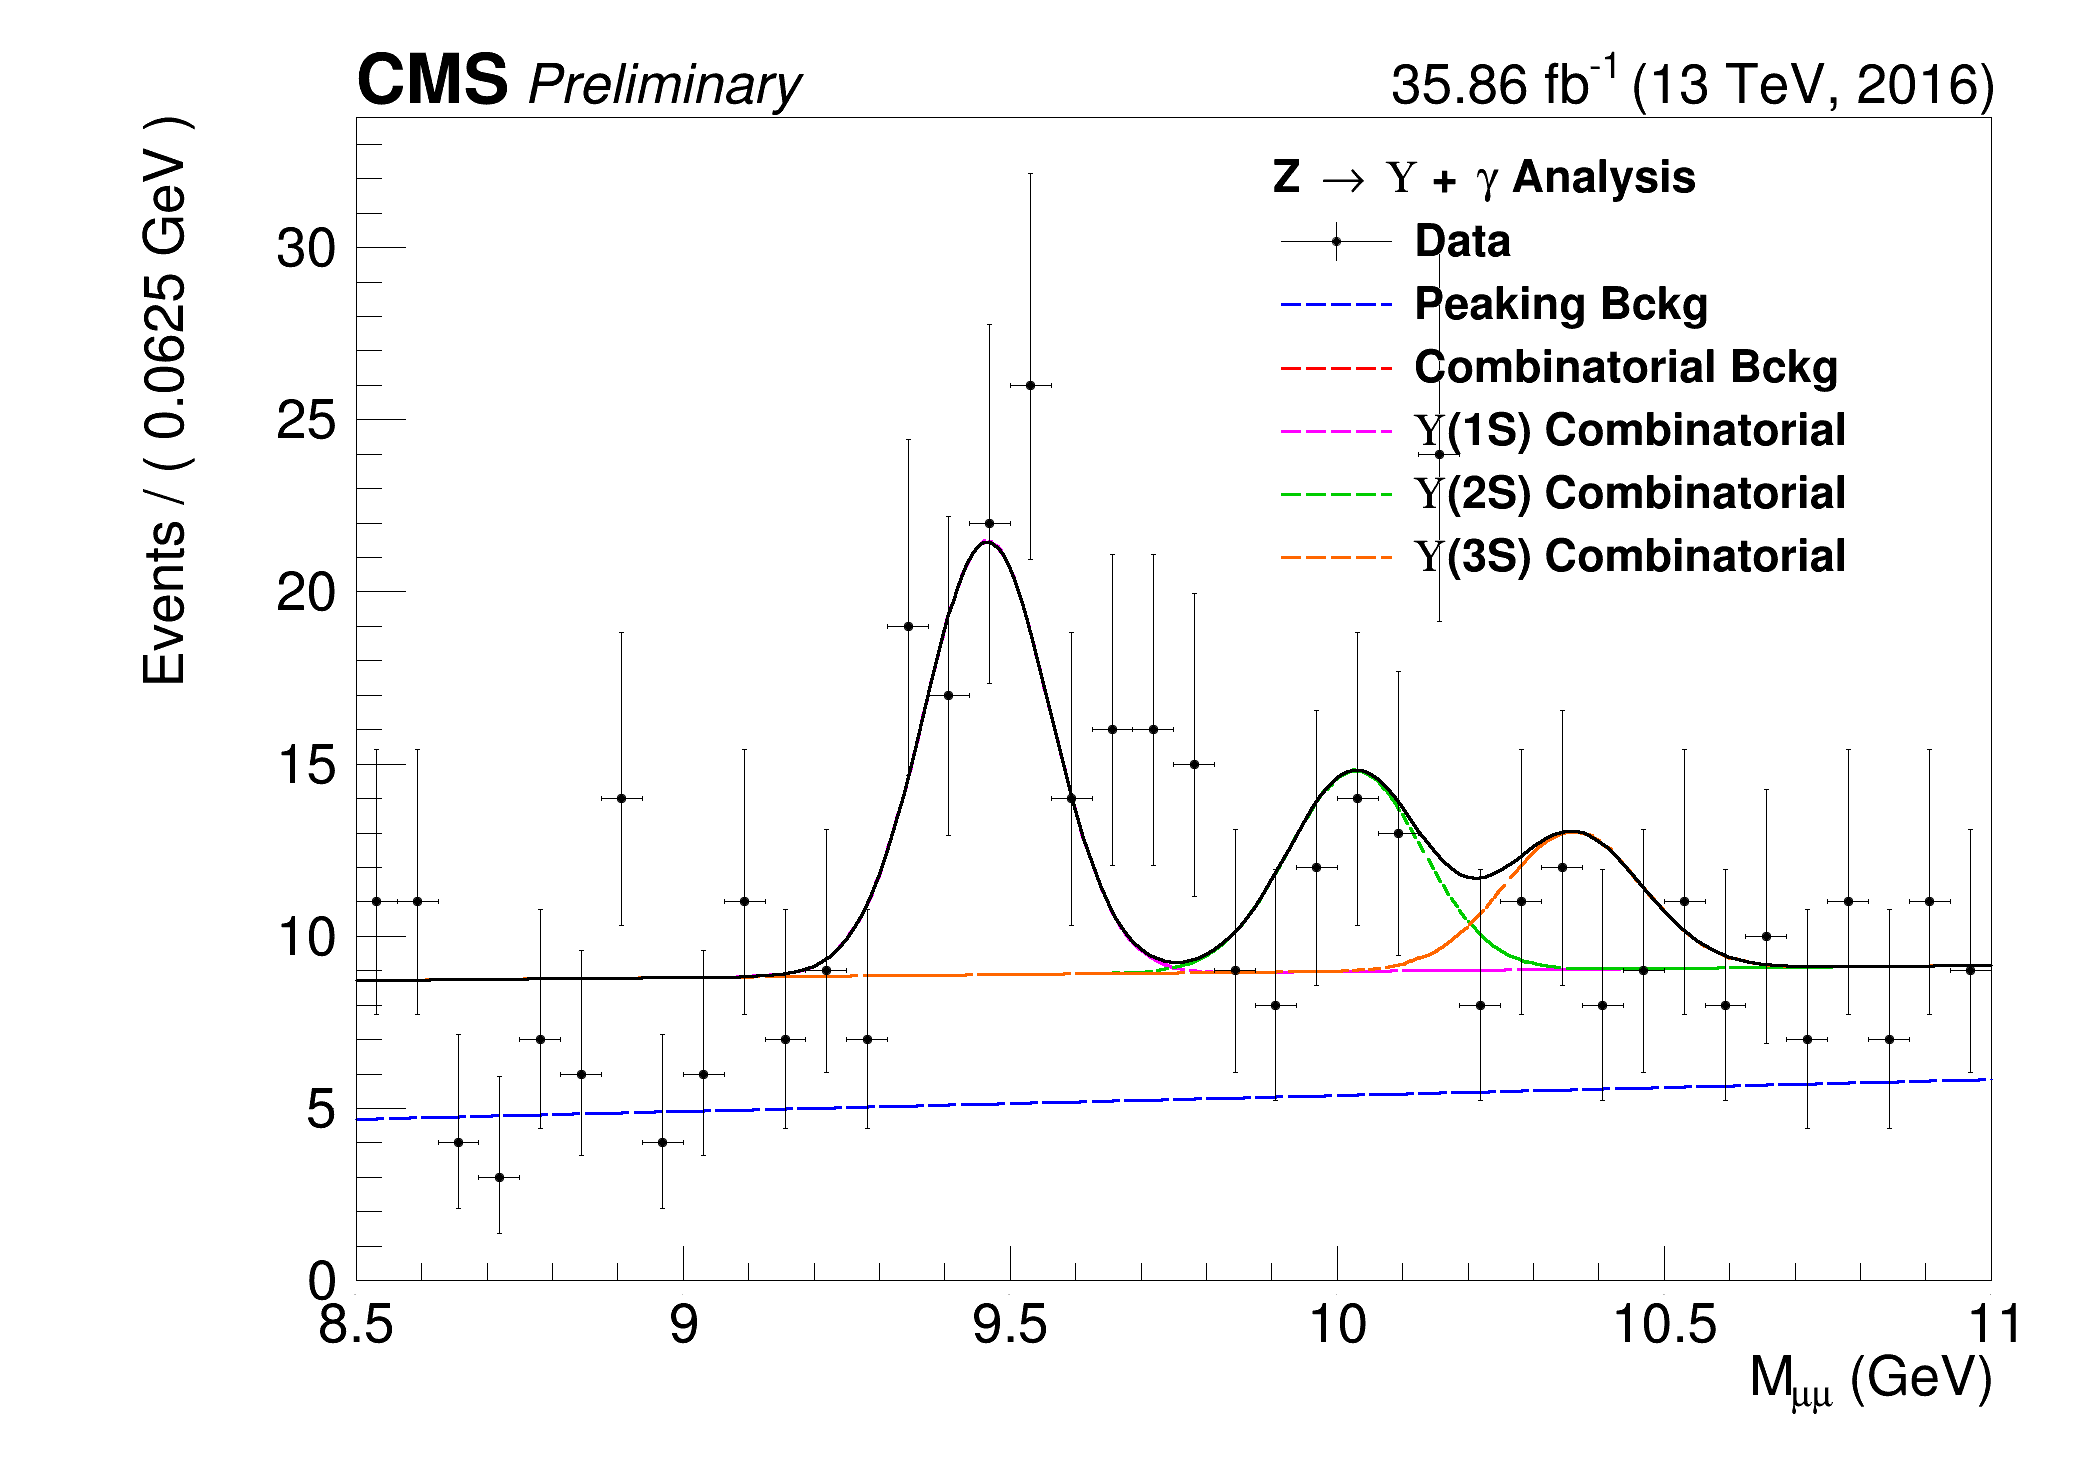
\includegraphics[width=0.45\textwidth]{figures_and_tables/fitPlotFiles2D/ftestOutput2D/outdir_ZToUpsilonPhoton_Cat0/bkgfTest-Data/mMuMU_multipdf_UntaggedTag_0}\hspace*{1.cm}
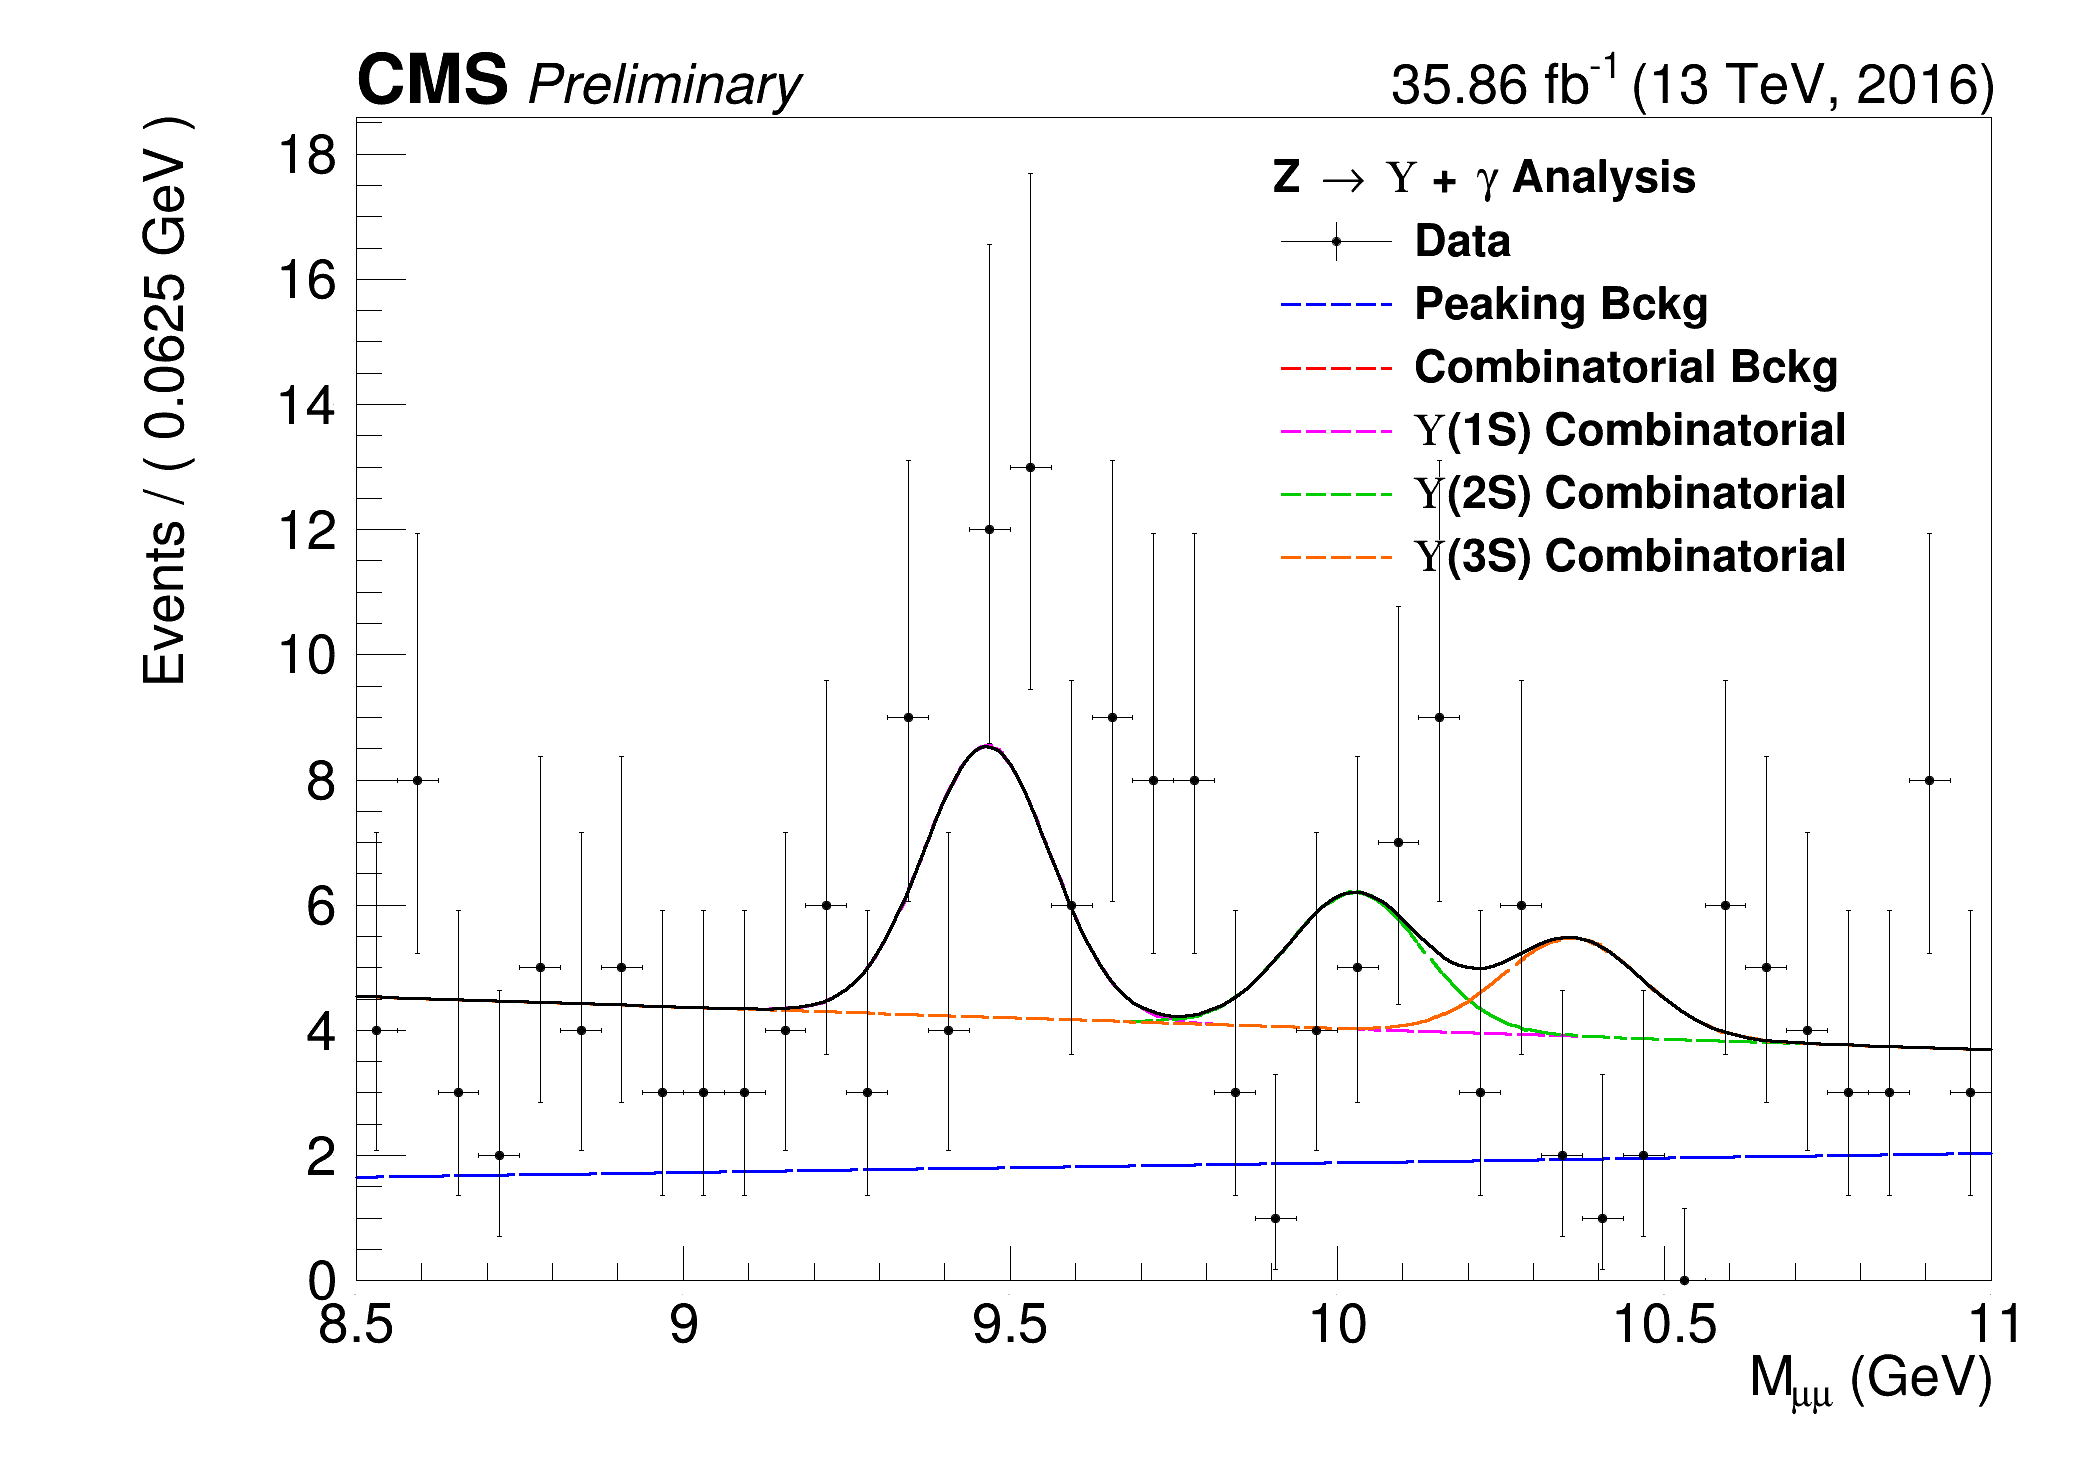
\includegraphics[width=0.45\textwidth]{figures_and_tables/fitPlotFiles2D/ftestOutput2D/outdir_ZToUpsilonPhoton_Cat1/bkgfTest-Data/mMuMU_multipdf_UntaggedTag_0}
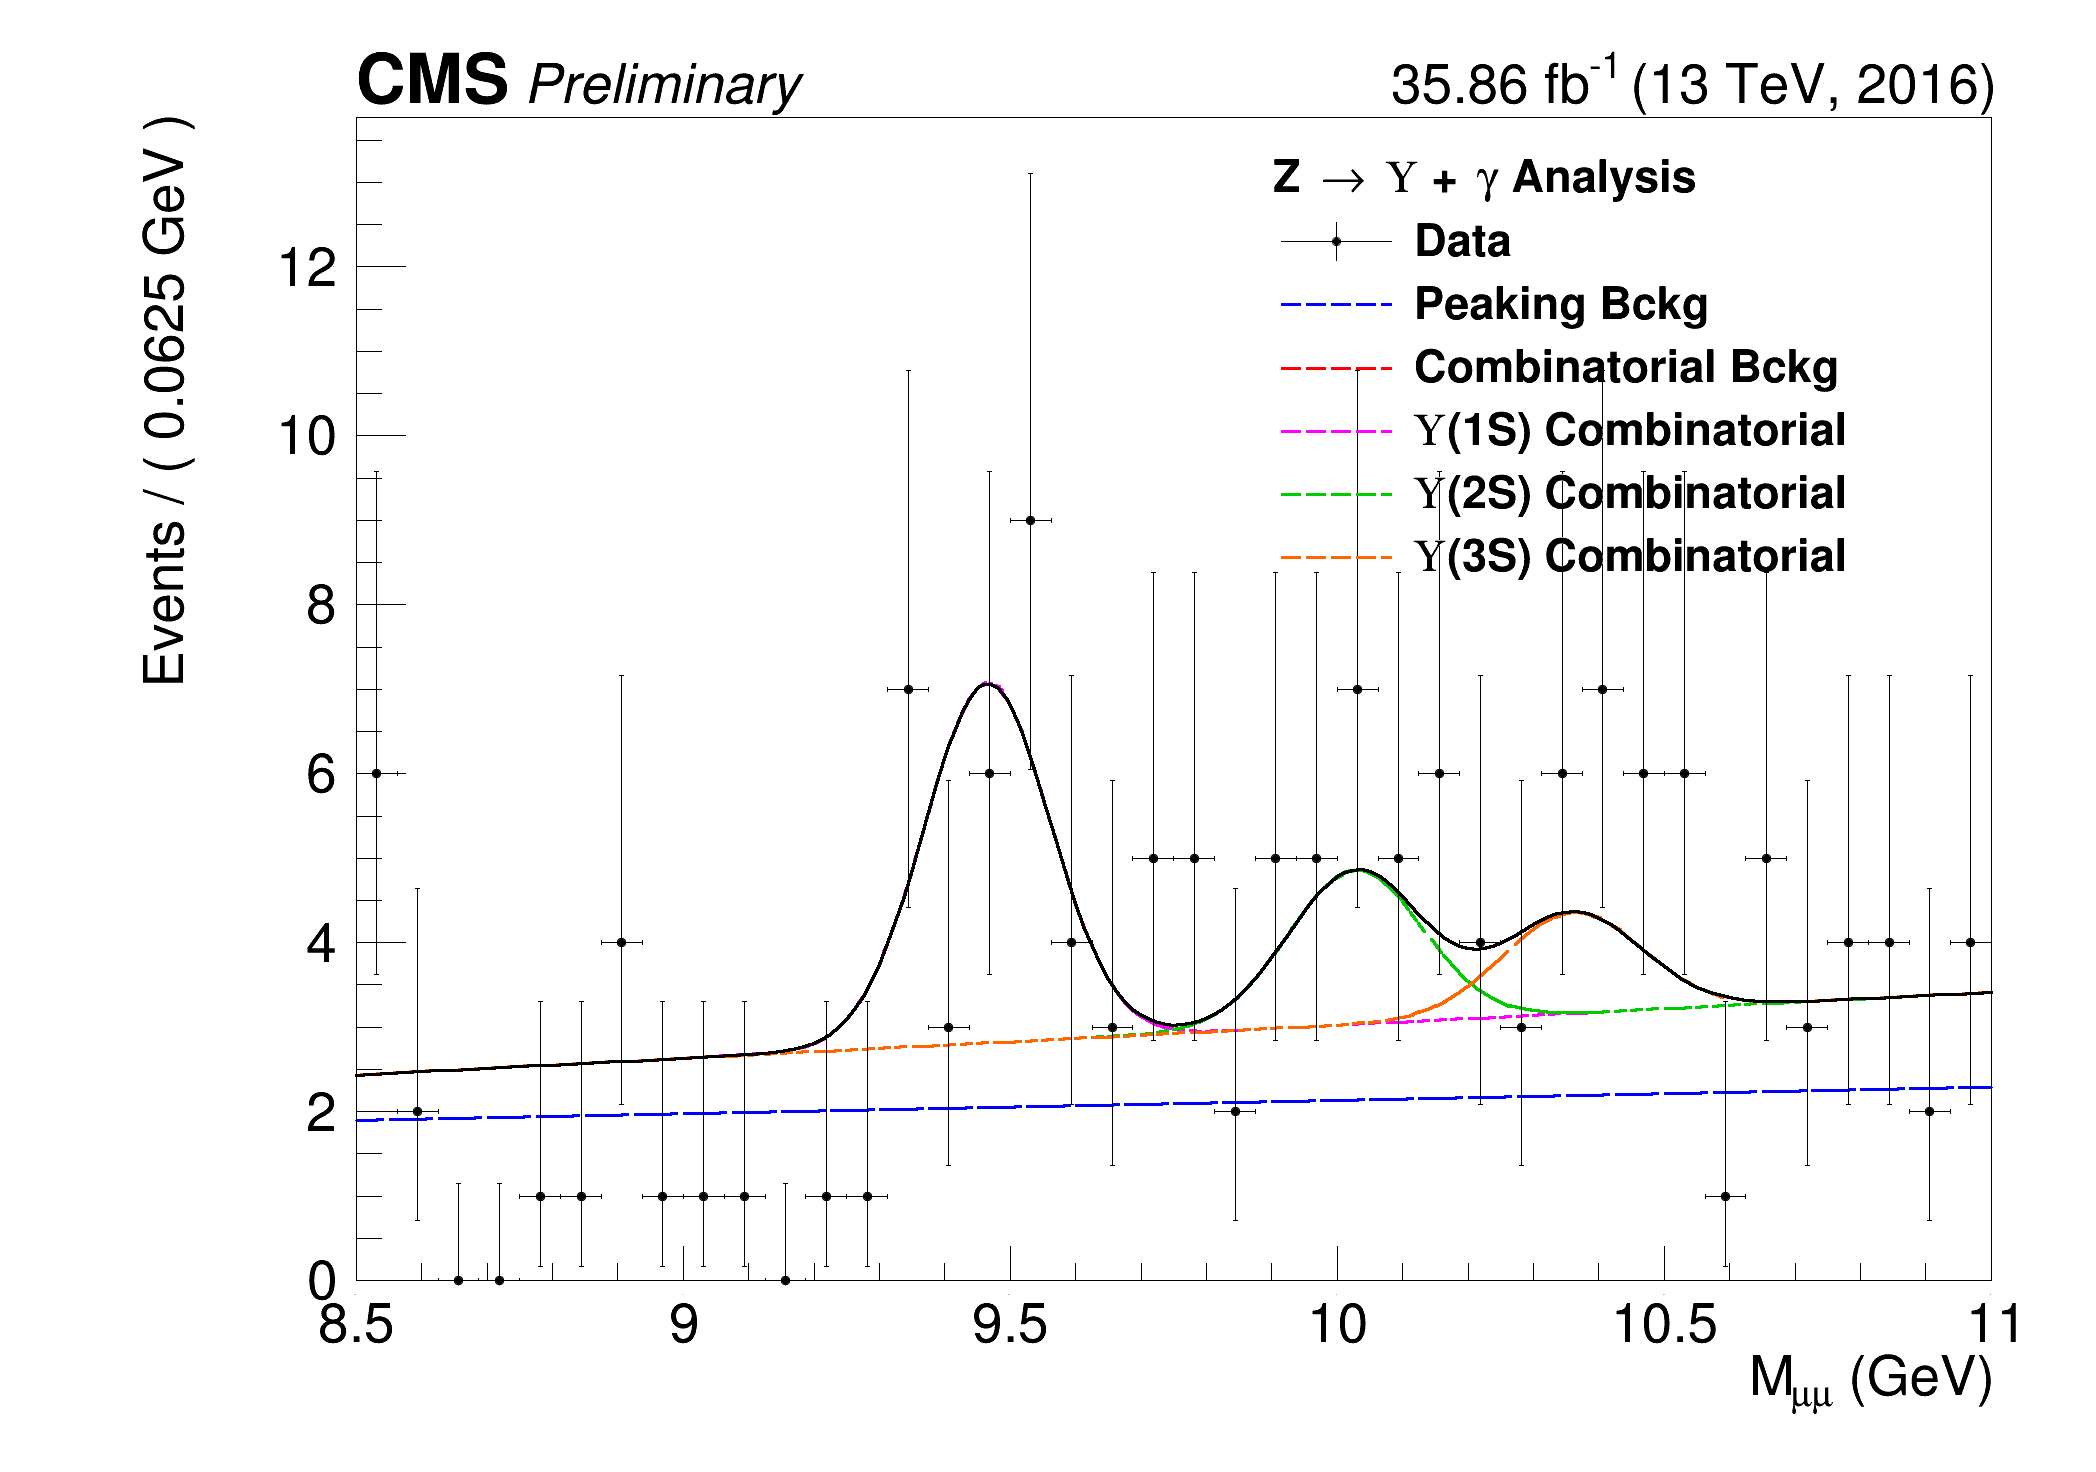
\includegraphics[width=0.45\textwidth]{figures_and_tables/fitPlotFiles2D/ftestOutput2D/outdir_ZToUpsilonPhoton_Cat2/bkgfTest-Data/mMuMU_multipdf_UntaggedTag_0}\hspace*{1.cm}
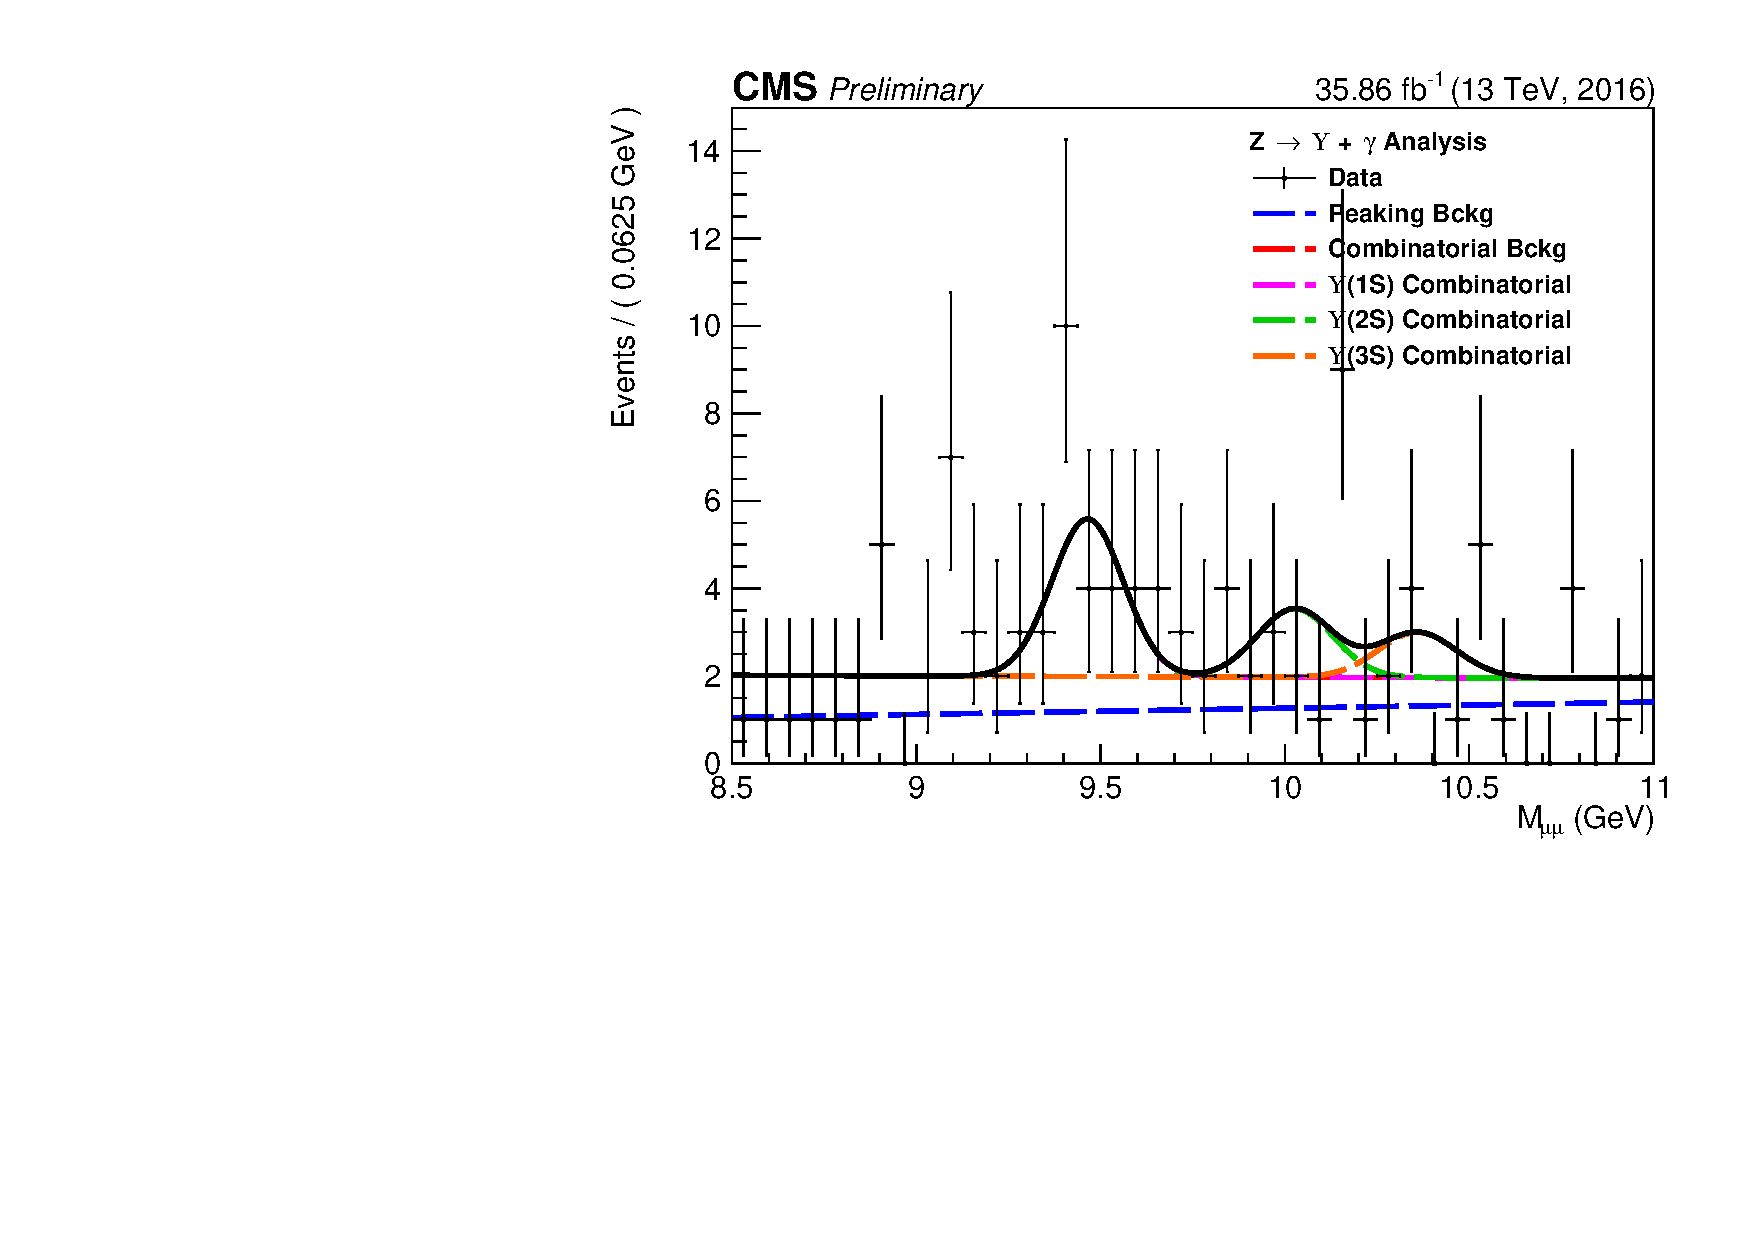
\includegraphics[width=0.45\textwidth]{figures_and_tables/fitPlotFiles2D/ftestOutput2D/outdir_ZToUpsilonPhoton_Cat3/bkgfTest-Data/mMuMU_multipdf_UntaggedTag_0}
\end{center}\vspace*{-.5cm}
\caption{$Z \rightarrow \Upsilon(1S,2S,3S) +\gamma$ Background Modeling: $\mu\mu$ distribution. Inclusive (top left); EB High R9 (top right), EB Low R9 (bottom left), EE (bottom right). The pdfs projections are plotted with respect to the overall best choice of the statistica test.}
\label{fig:ZToUpsilon_mMuMU_Projection}
\end{figure}

%%%%%%%%%%%%

% Z To Upsilon - mHZ Projection
\begin{figure}[!htbp]
\begin{center}
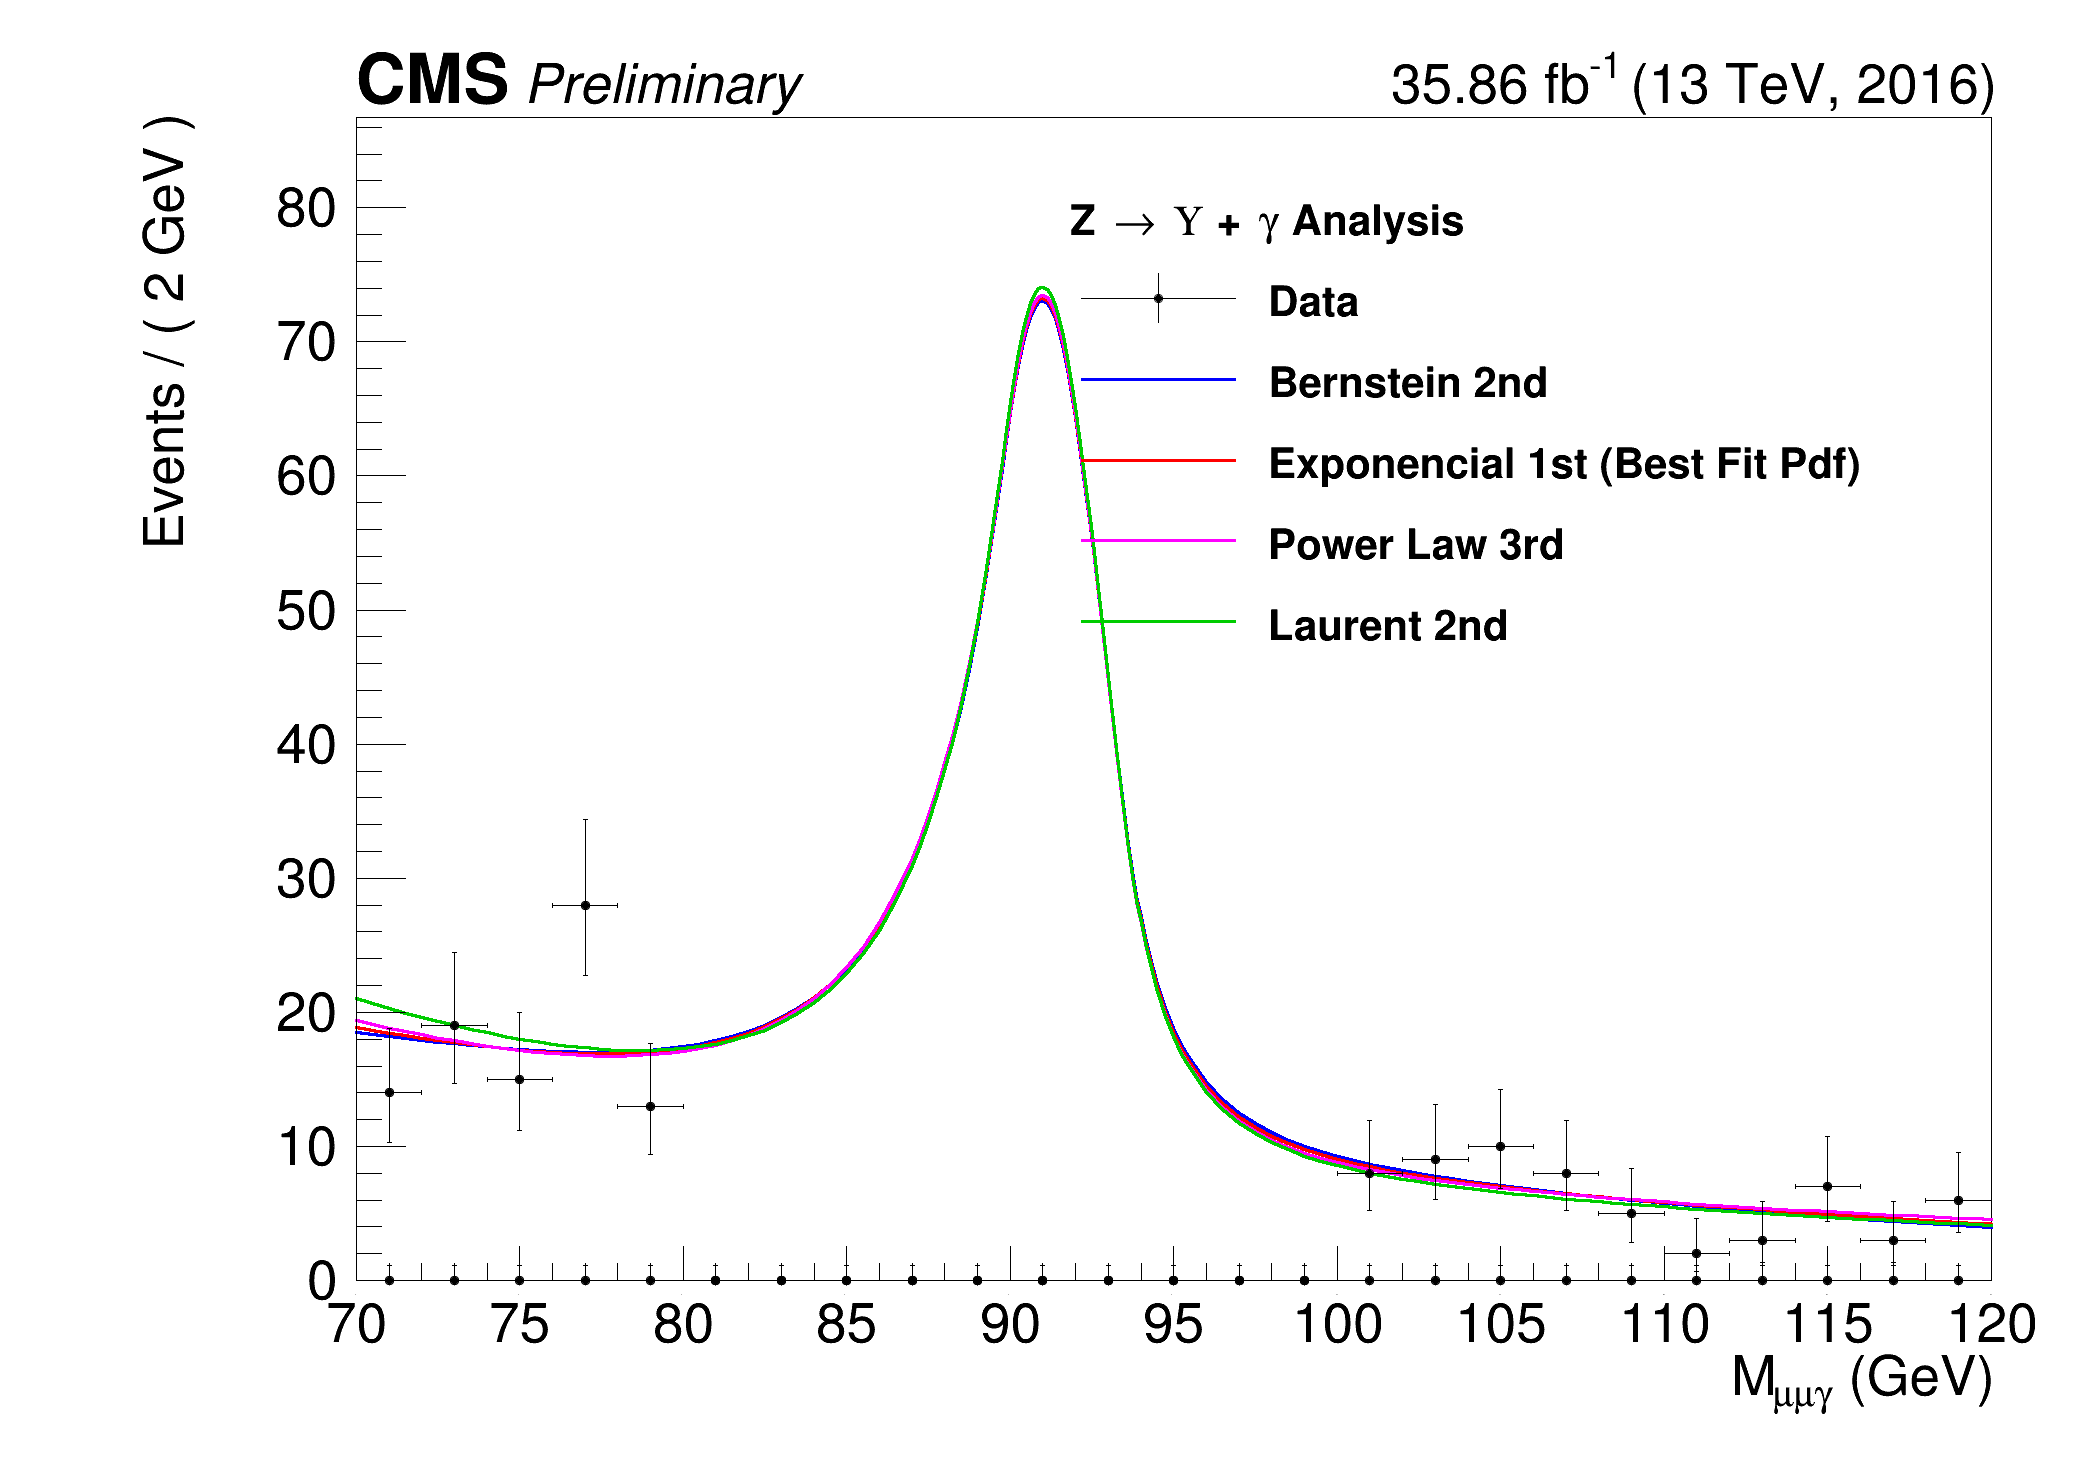
\includegraphics[width=0.45\textwidth]{figures_and_tables/fitPlotFiles2D/ftestOutput2D/outdir_ZToUpsilonPhoton_Cat0/bkgfTest-Data/mHZ_multipdf_UntaggedTag_0}\hspace*{1.cm}
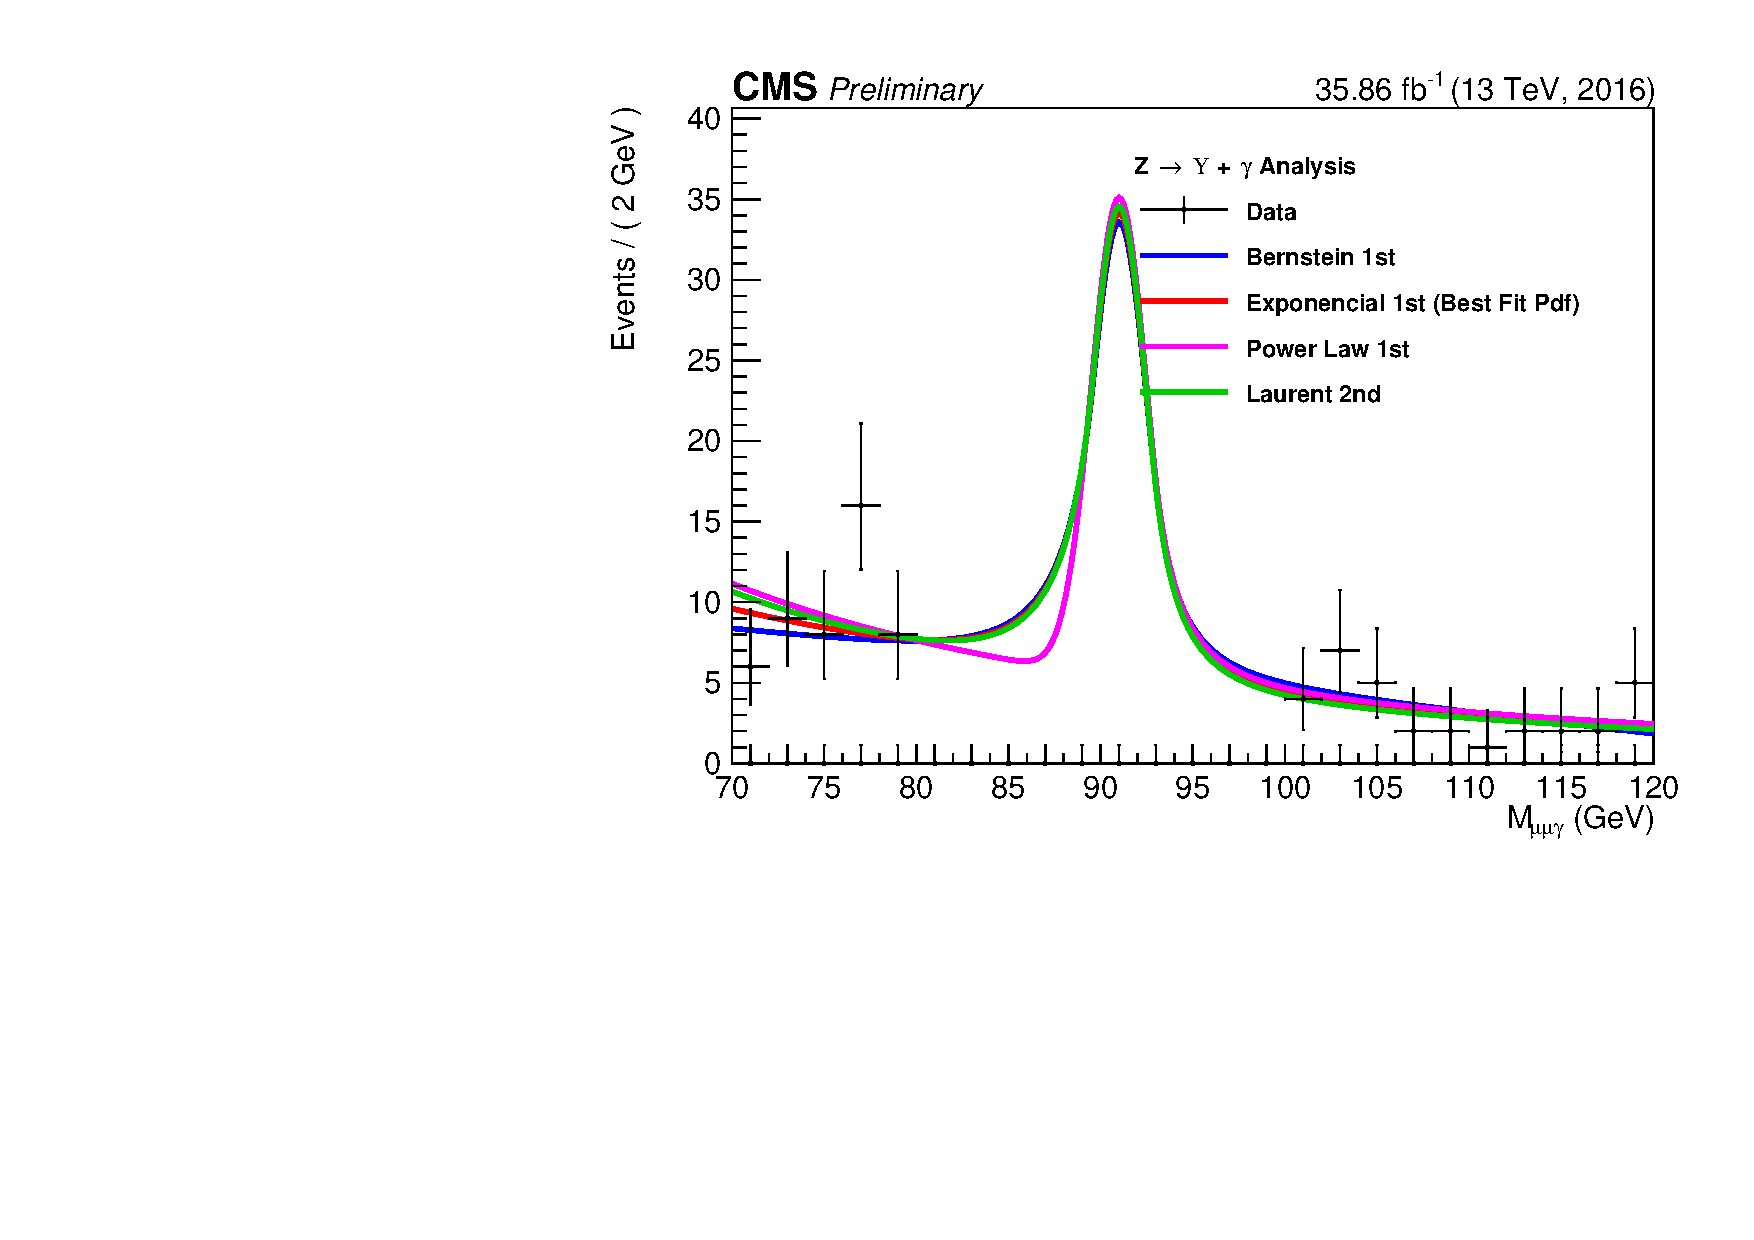
\includegraphics[width=0.45\textwidth]{figures_and_tables/fitPlotFiles2D/ftestOutput2D/outdir_ZToUpsilonPhoton_Cat1/bkgfTest-Data/mHZ_multipdf_UntaggedTag_0}
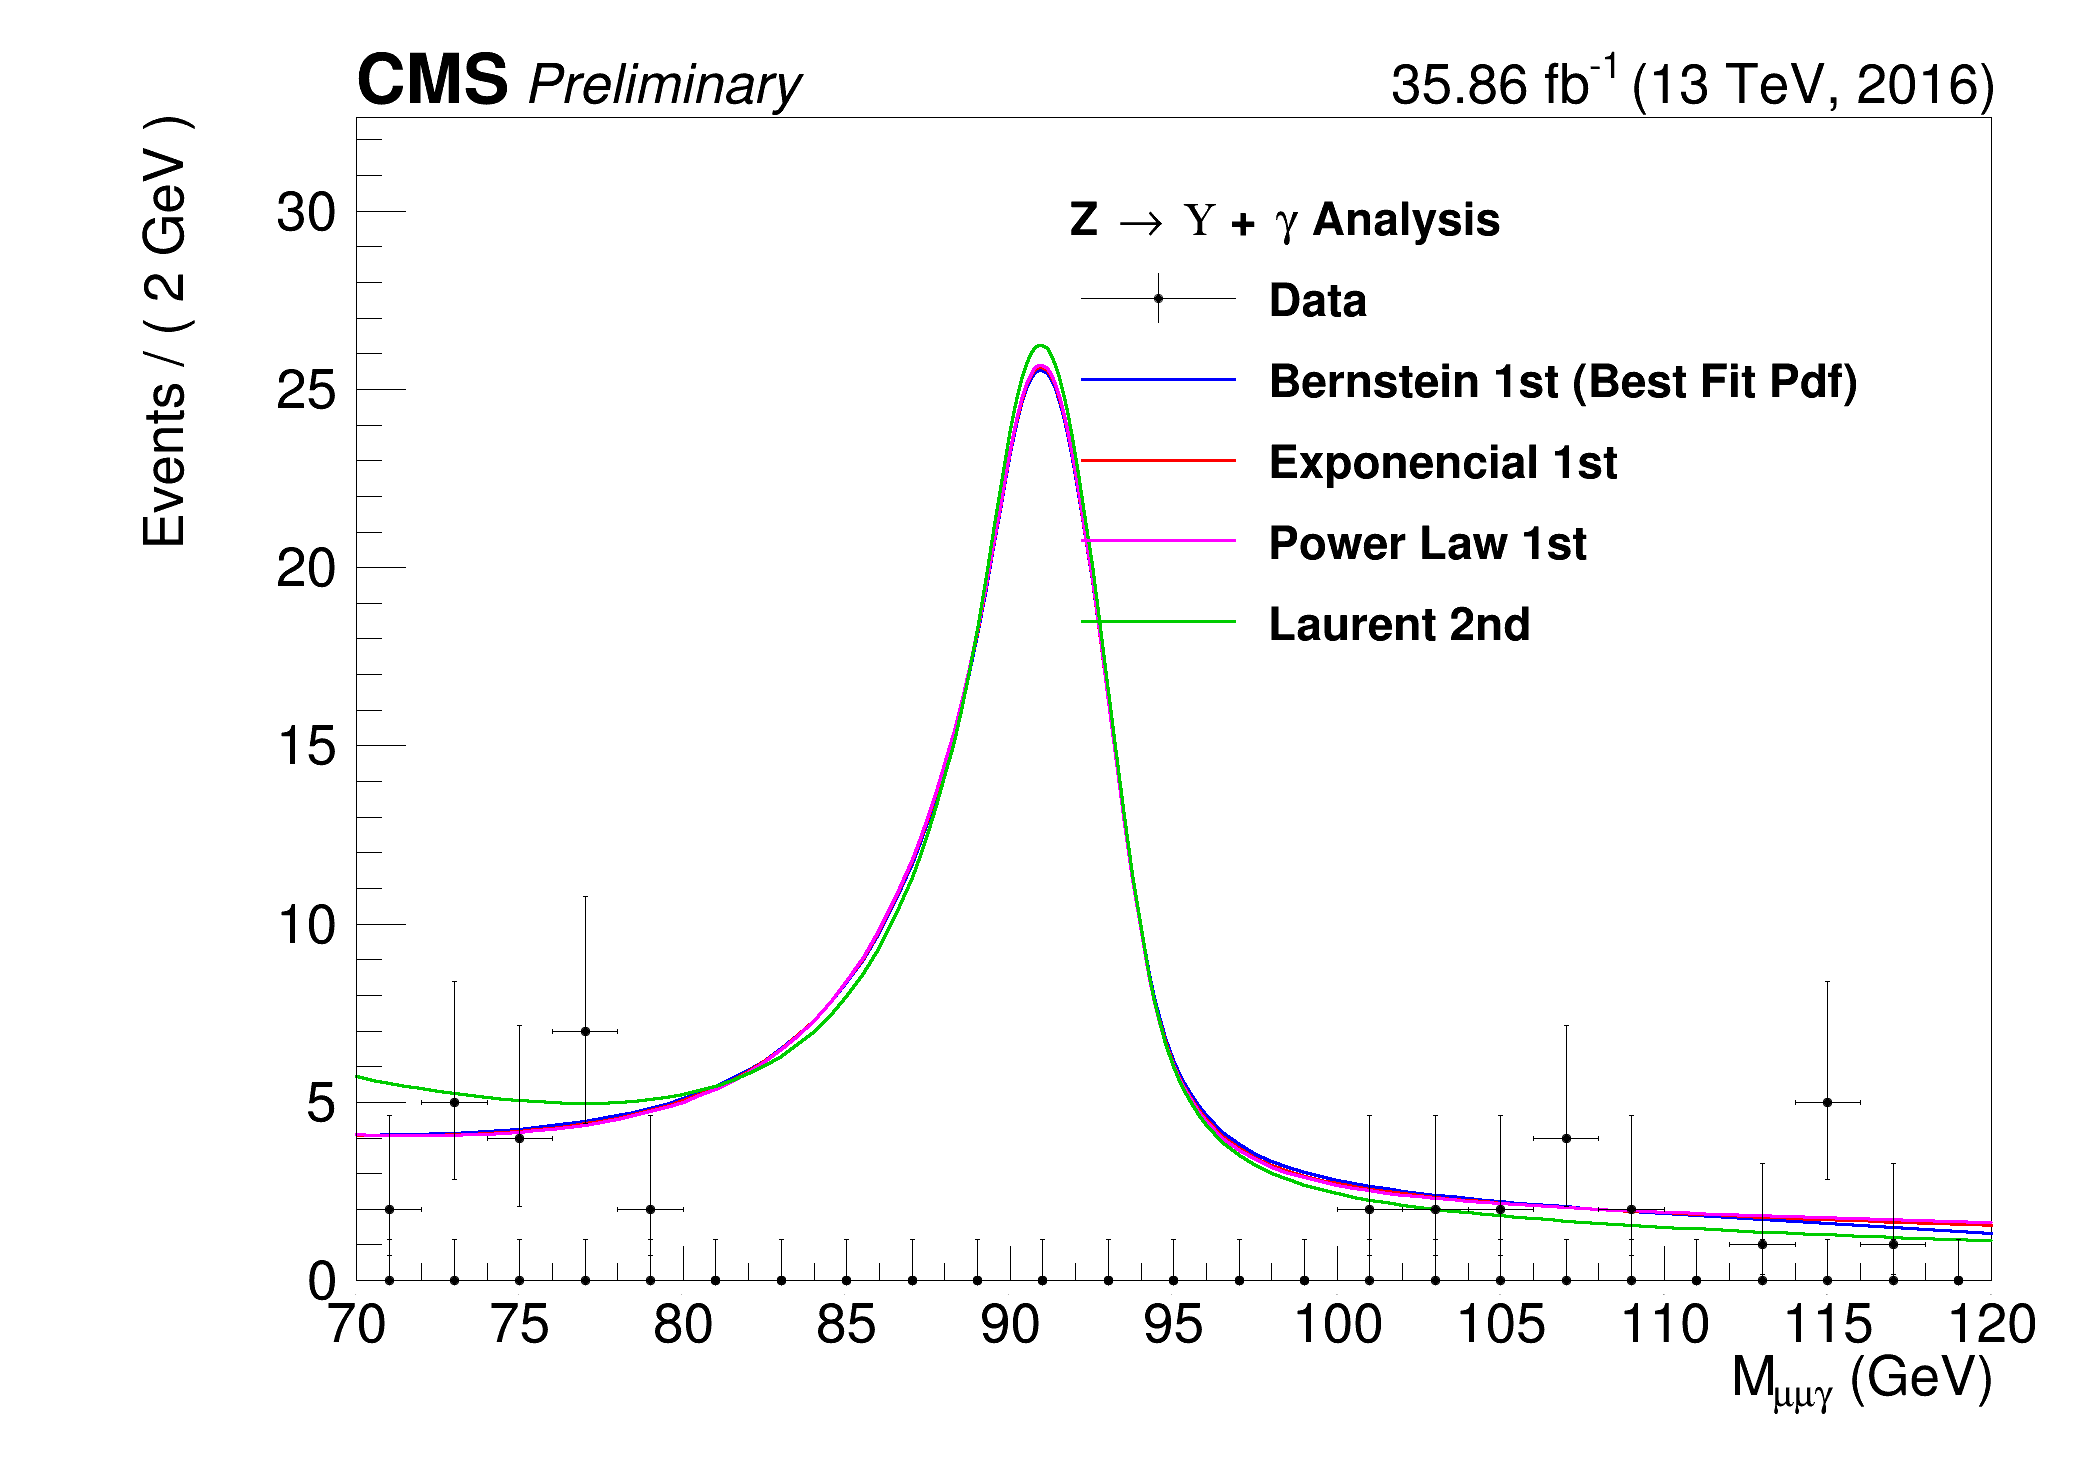
\includegraphics[width=0.45\textwidth]{figures_and_tables/fitPlotFiles2D/ftestOutput2D/outdir_ZToUpsilonPhoton_Cat2/bkgfTest-Data/mHZ_multipdf_UntaggedTag_0}\hspace*{1.cm}
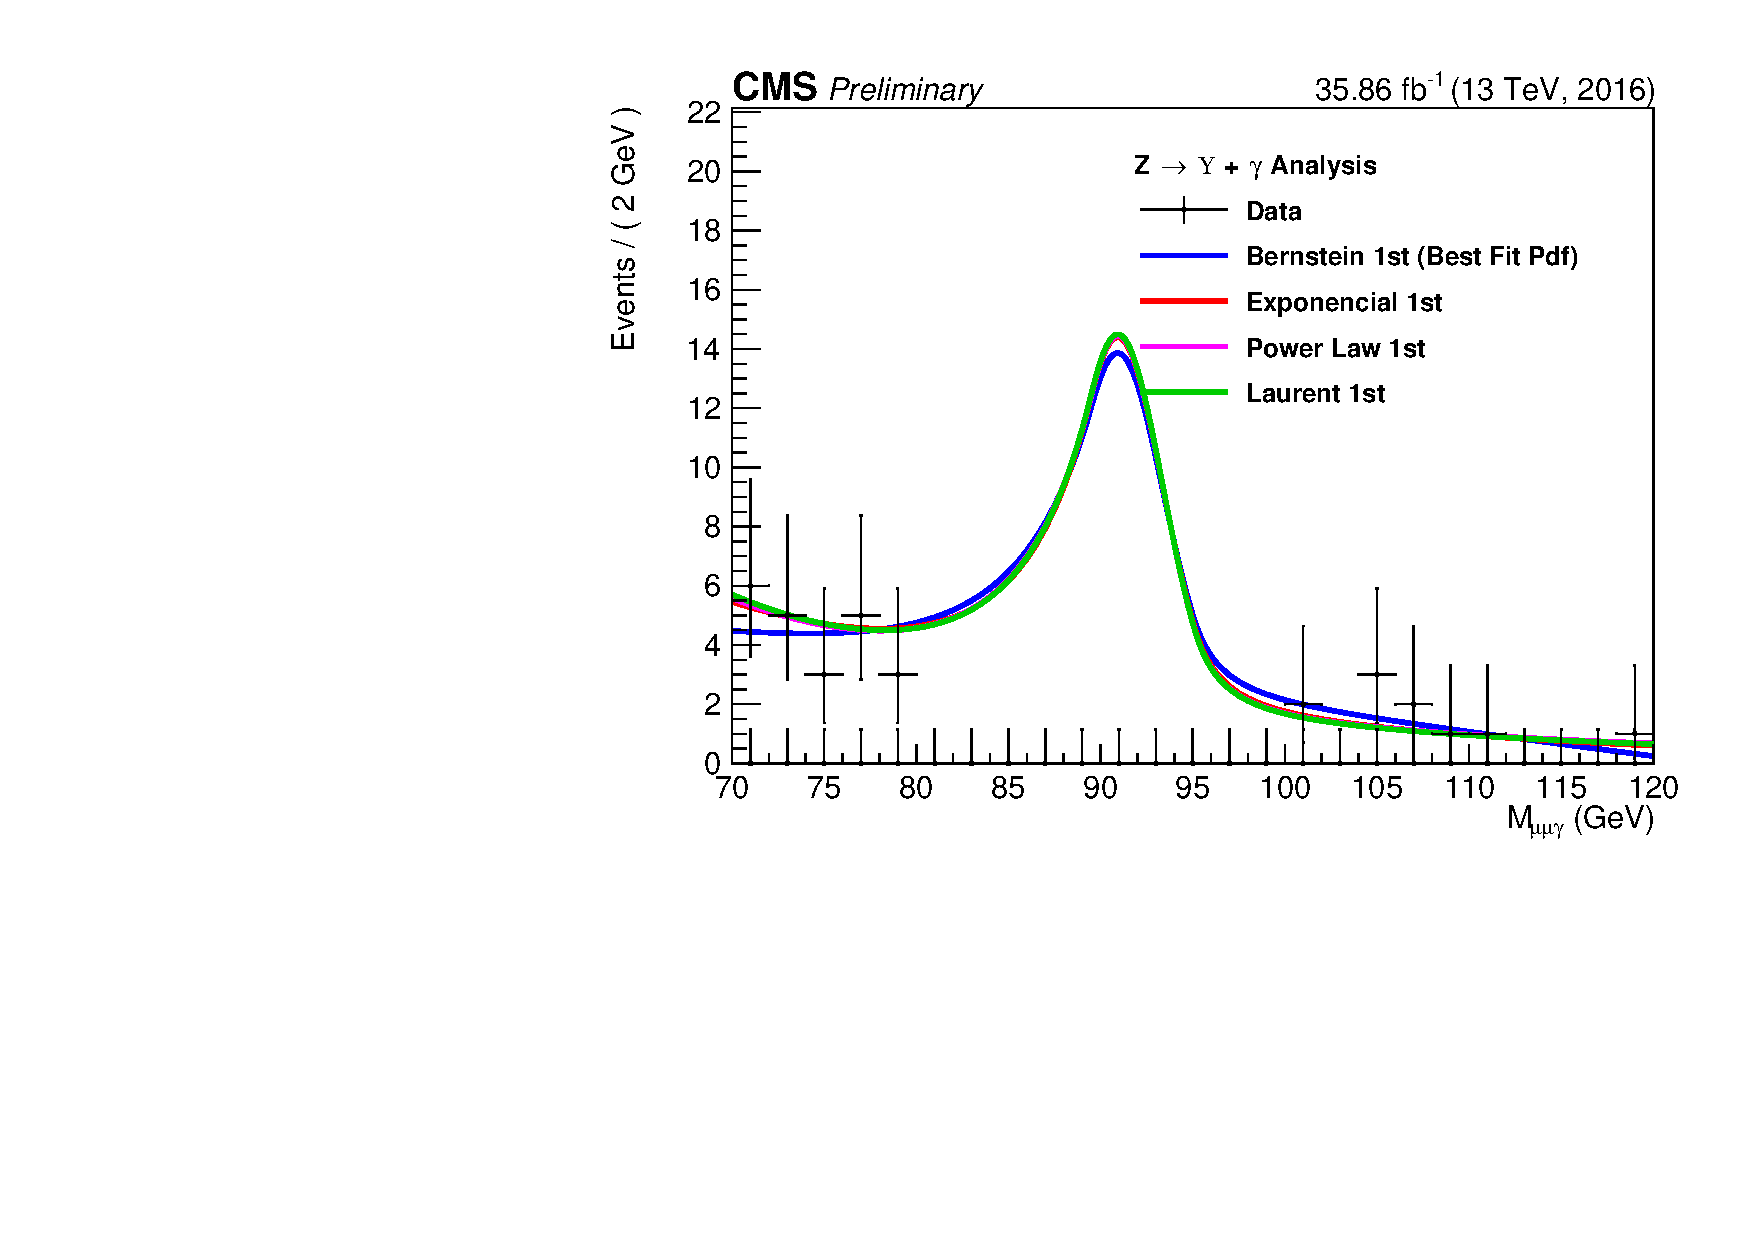
\includegraphics[width=0.45\textwidth]{figures_and_tables/fitPlotFiles2D/ftestOutput2D/outdir_ZToUpsilonPhoton_Cat3/bkgfTest-Data/mHZ_multipdf_UntaggedTag_0}
\end{center}\vspace*{-.5cm}
\caption{$Z \rightarrow \Upsilon(1S,2S,3S) +\gamma$ Background Modeling: $\mu\mu\gamma$ distribution. Inclusive (top left); EB High R9 (top right), EB Low R9 (bottom left), EE (bottom right). The plotted \textit{pdfs} corresponds to the best choice by the statistical test for each family. The signal region, from 80 GeV to 100 GeV was blinded.}
\label{fig:ZToUpsilon_mHZ_Projection}
\end{figure}


For the $H \rightarrow \Upsilon(1S,2S,3S) + \gamma$ analysis, the same procedure is implemented, except for the resonant background modeling. Since the MC prediction for the contribution of the background is too small, according to the comparison between the final selected events for data and the Higgs Dalitz Decay sample, in order to avoid fitting over statistical fluctuations of the data sample, the Resonant Background, for the Higgs channel, is fully modeled from the MC sample, including its normalization, as shown in figure \ref{fig:HToUpsilon_PeakingBackground}, hence it is not includedthestatistical test, neither in the final background modeling envelope.

The results of the background modeling for the Full Combinatorial and $\Upsilon$ Combinatorial, can be found at Figures \ref{fig:HToUpsilon_mMuMU_Projection} and \ref{fig:HToUpsilon_mHZ_Projection}, for the $\mu\mu$ and $\mu\mu\gamma$ distribution, respectively. It is worth to remember that, for the Higgs channel, we are not implementing any categorization.


% H To Upsilon - peaking background
\begin{figure}[!htbp]
\begin{center}
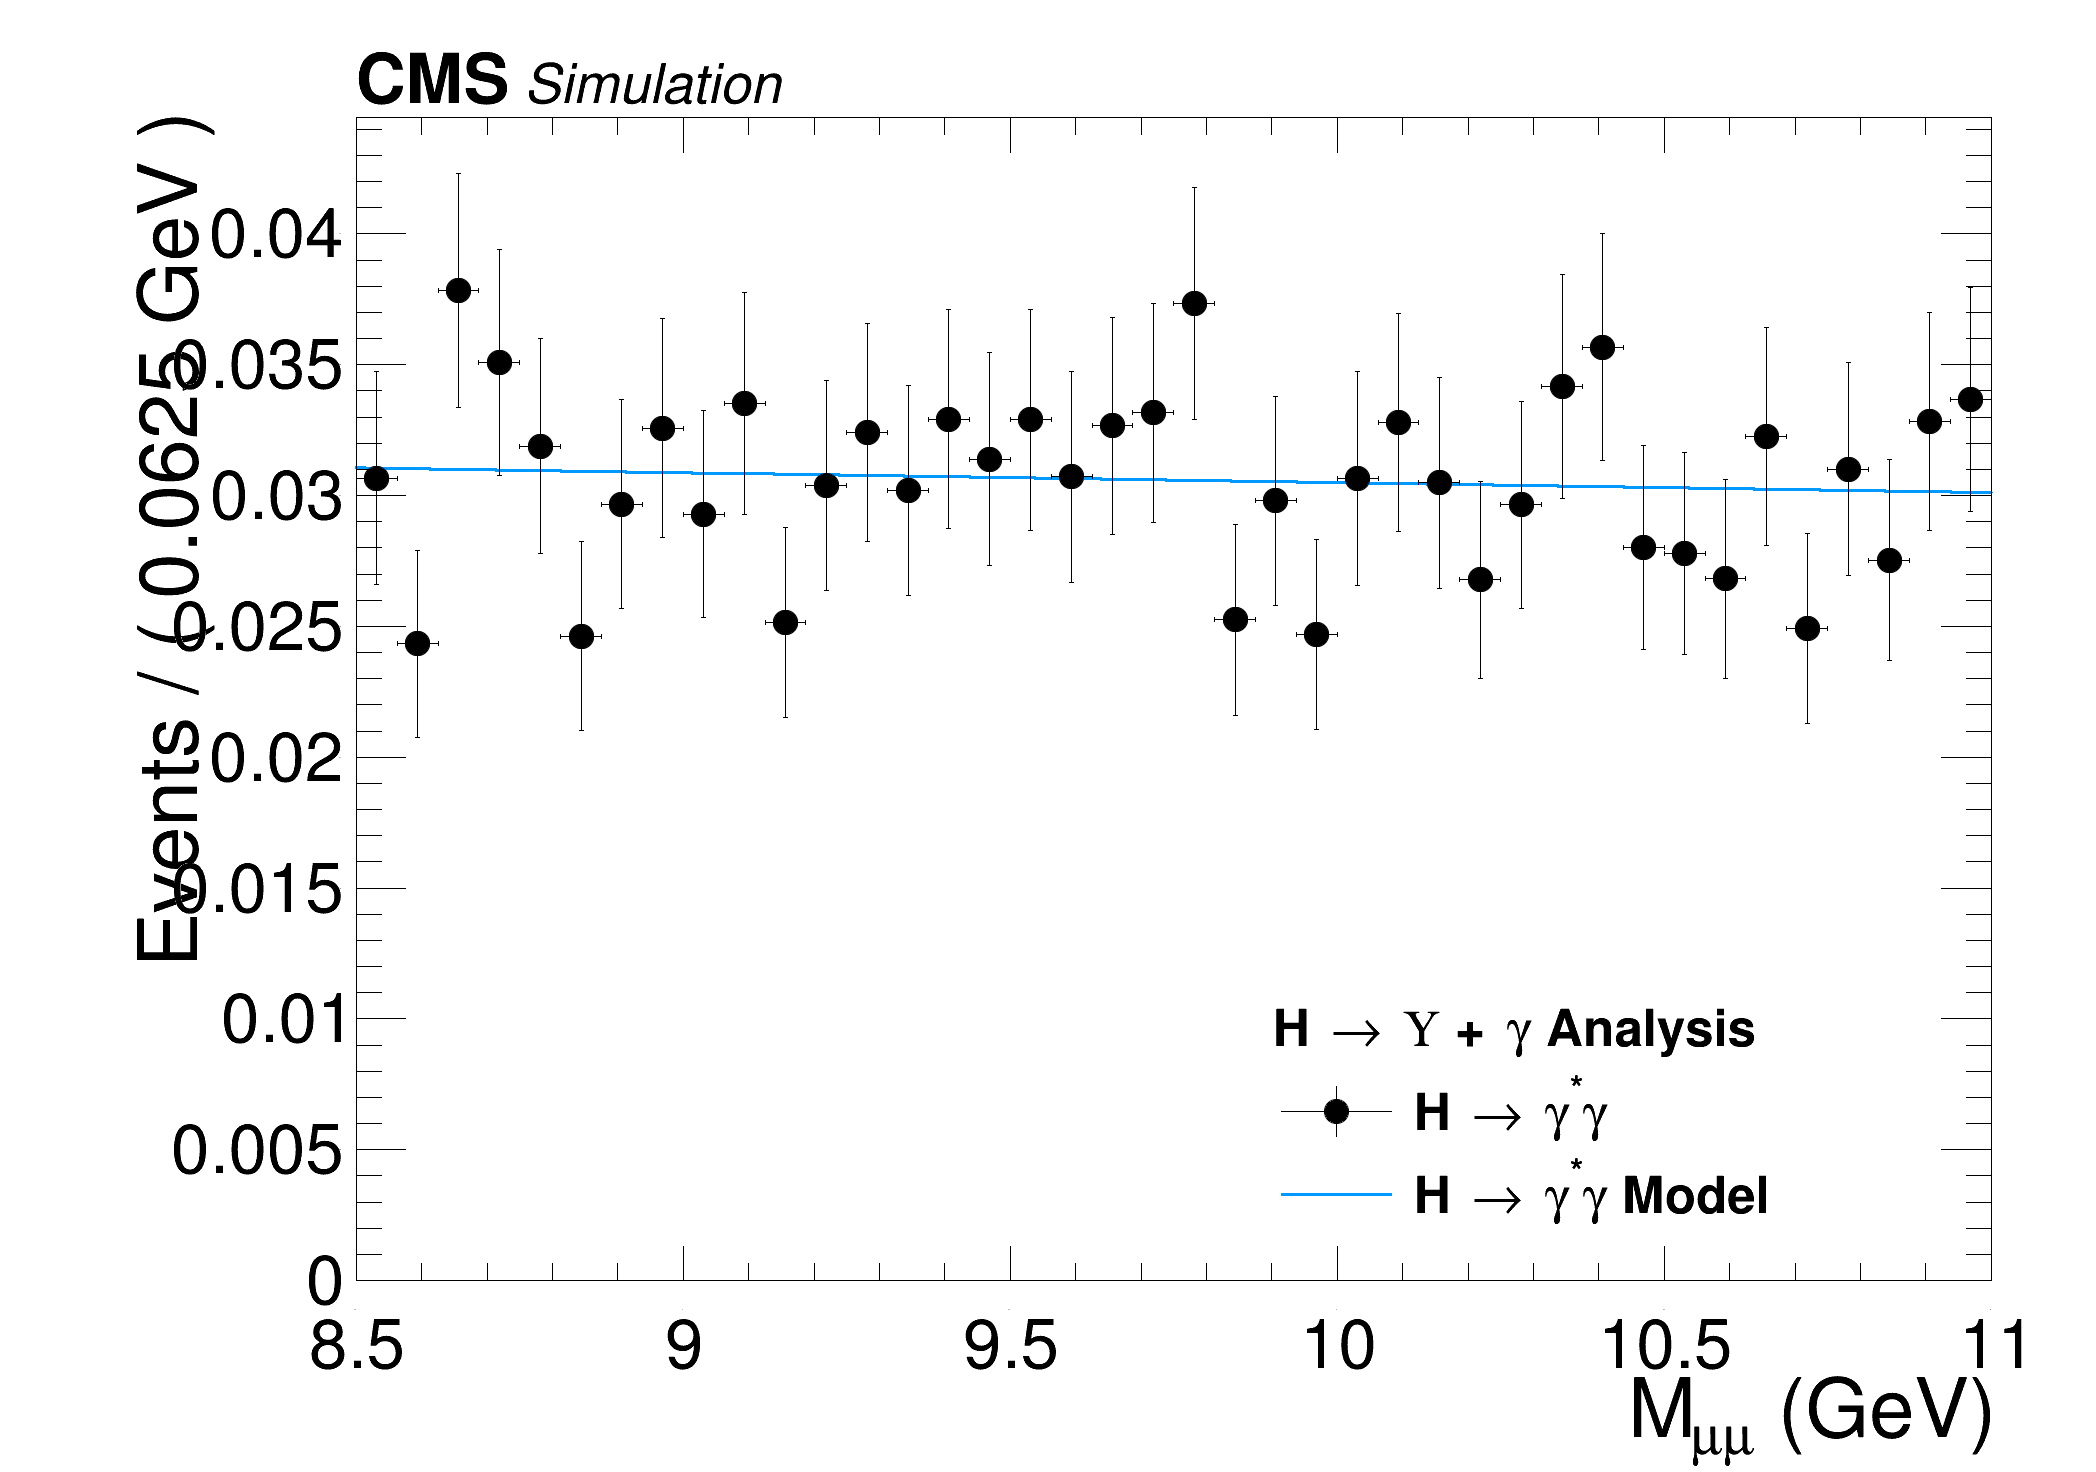
\includegraphics[width=0.45\textwidth]{figures_and_tables/fitPlotFiles2D/HToUpsilonPhotonSignalAndBackgroundFit/mMuMNU_HToUpsilon1SPhotonSignalAndBackgroundFit_PeakingBackground_Cat0}\hspace*{1.cm}
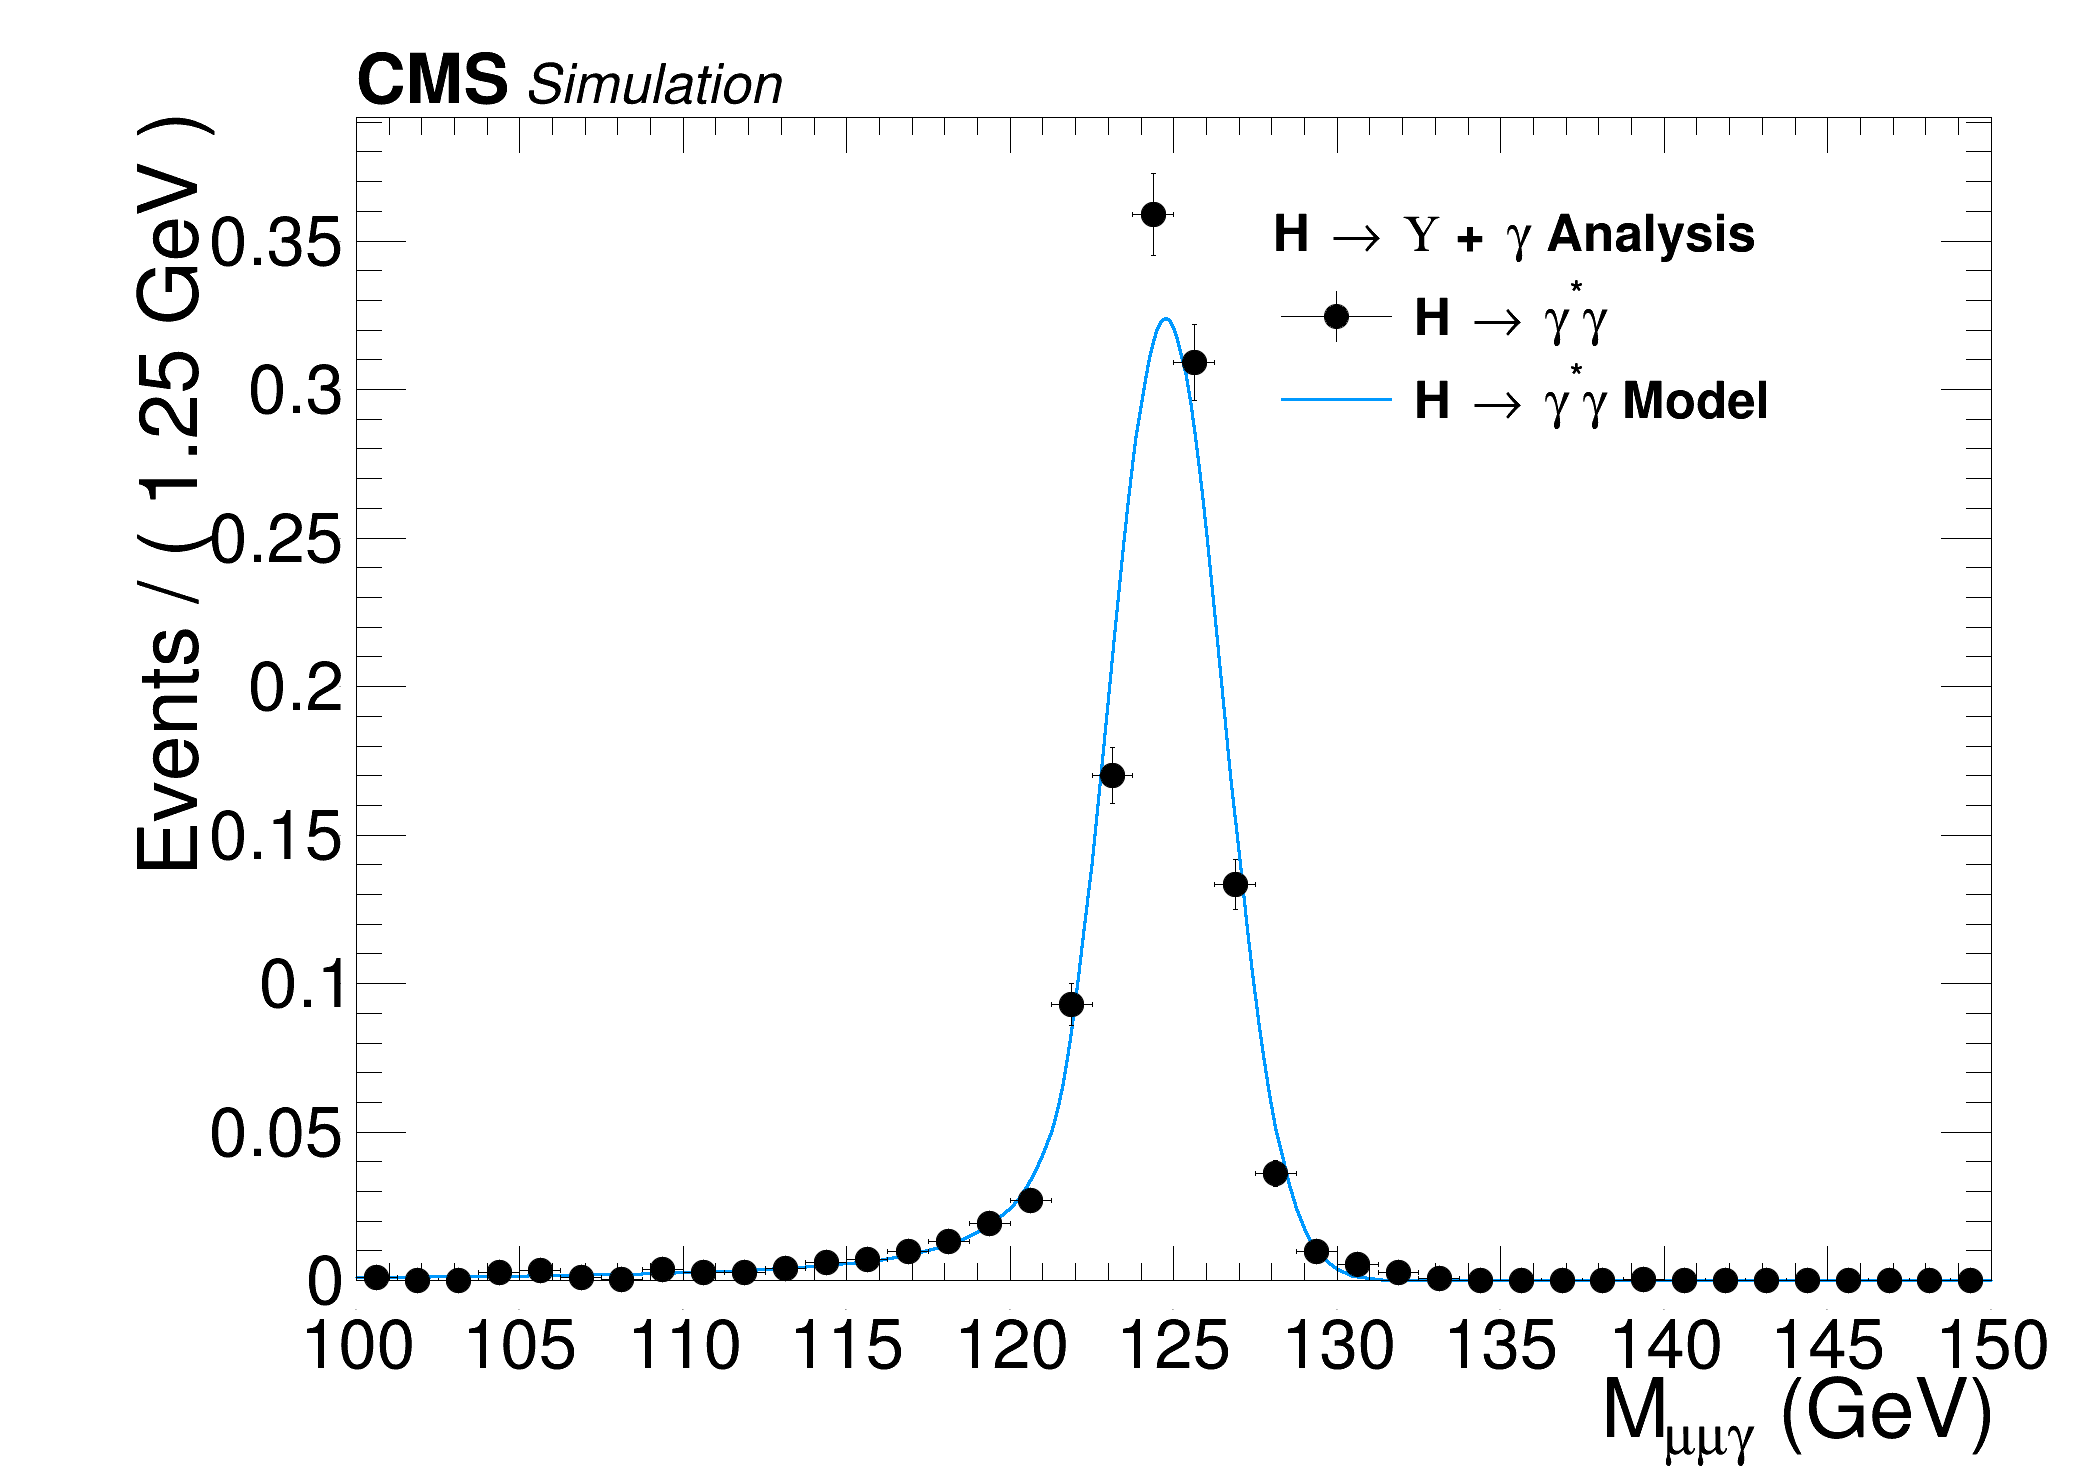
\includegraphics[width=0.45\textwidth]{figures_and_tables/fitPlotFiles2D/HToUpsilonPhotonSignalAndBackgroundFit/mHZ_HToUpsilon1SPhotonSignalAndBackgroundFit_PeakingBackground_Cat0}\hspace*{1.cm}
\end{center}\vspace*{-.5cm}
\caption{Resonant Background for the $H \rightarrow \Upsilon(1S,2S,3S) +\gamma$ analysis. $m_{\mu\mu}$ invariant mass distribution (left) and $m_{\mu\mu\gamma}$ invariant mass distribution (right).}
\label{fig:HToUpsilon_PeakingBackground}
\end{figure}


% H To Upsilon - mMuMU Projection
\begin{figure}[!htbp]
\begin{center}
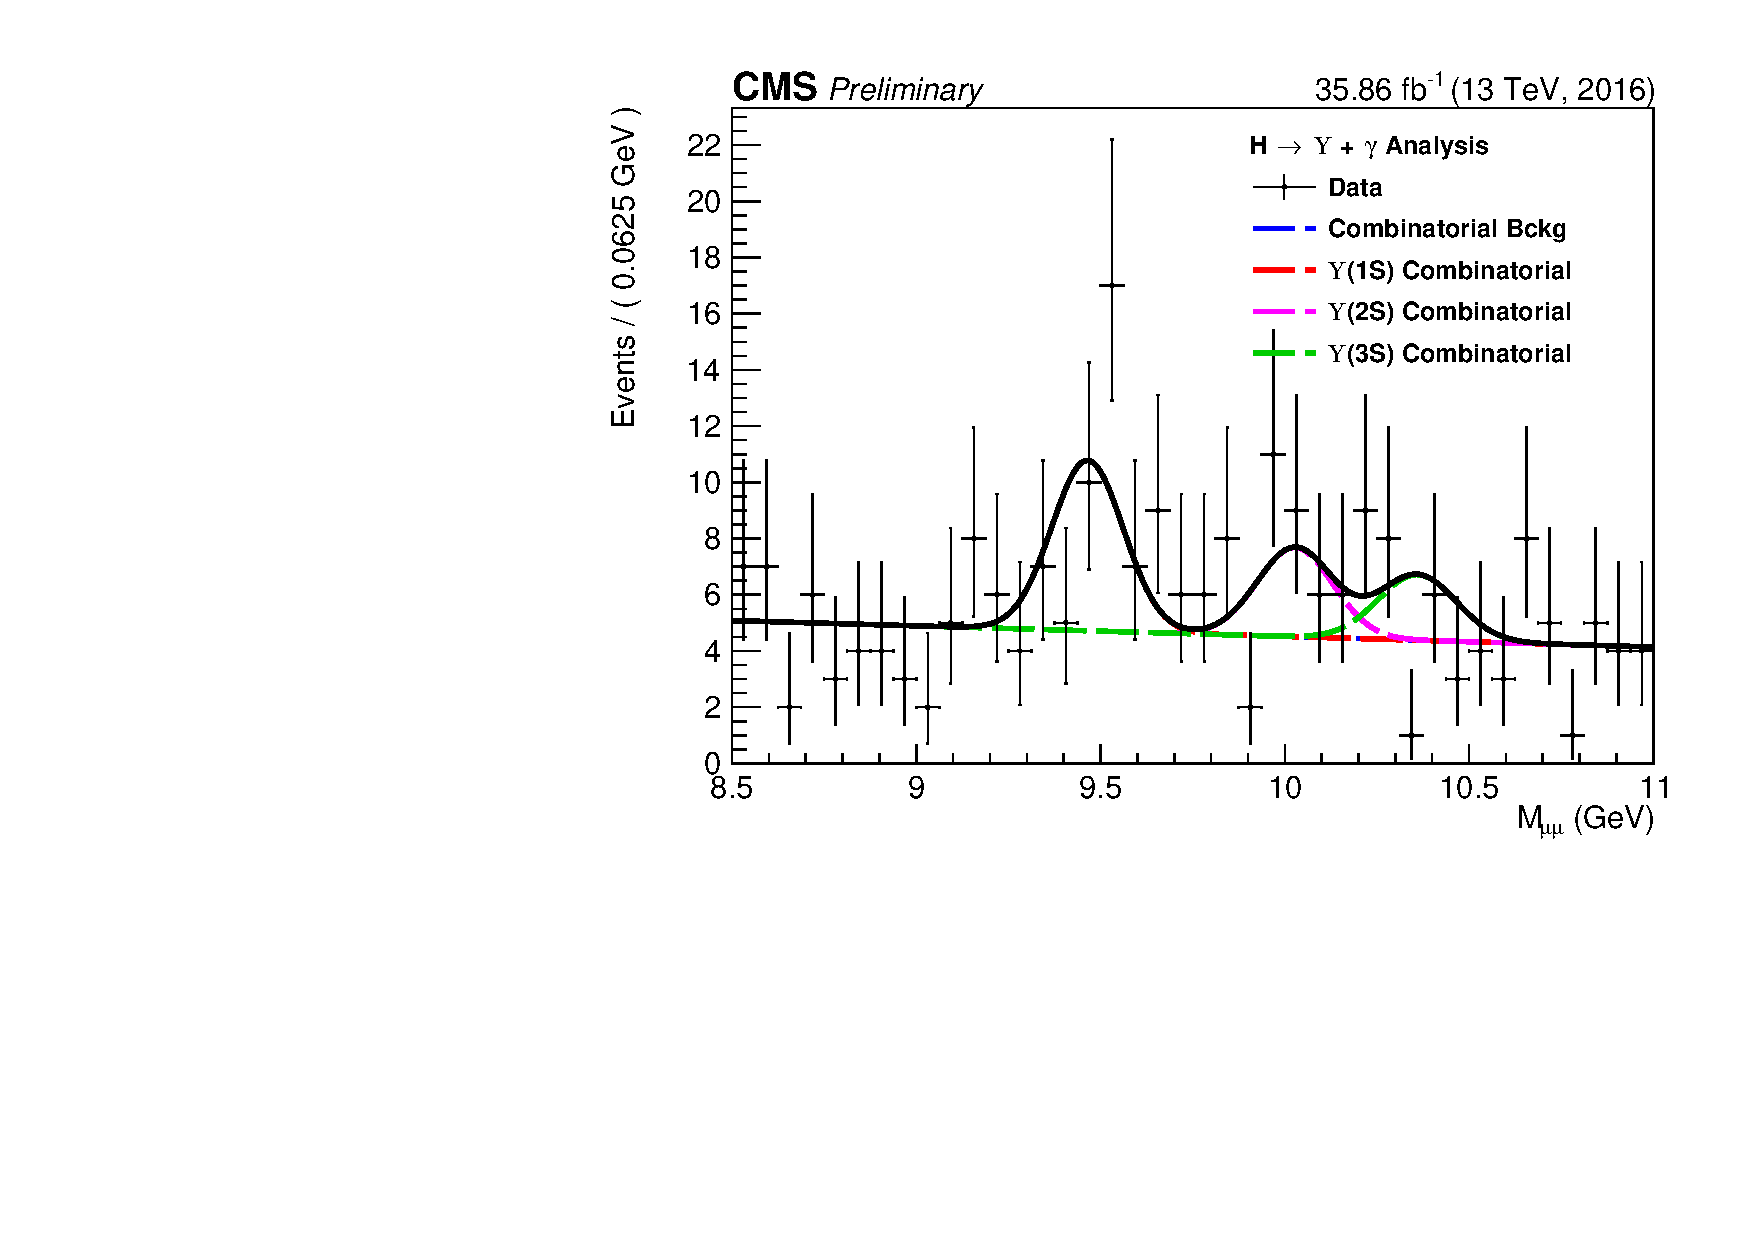
\includegraphics[width=0.45\textwidth]{figures_and_tables/fitPlotFiles2D/ftestOutput2D/outdir_HToUpsilonPhoton_Cat0/bkgfTest-Data/mMuMU_multipdf_UntaggedTag_0}\hspace*{1.cm}
\end{center}\vspace*{-.5cm}
\caption{$H \rightarrow \Upsilon(1S,2S,3S) +\gamma$ Background Modeling: $m_{\mu\mu}$ distribution. The \textit{pdfs} projections are plotted with respect to the overall best choice of the statistical test.}
\label{fig:HToUpsilon_mMuMU_Projection}
\end{figure}

%%%%%%%%%%%%

% H To Upsilon - mHZ Projection
\begin{figure}[!htbp]
\begin{center}
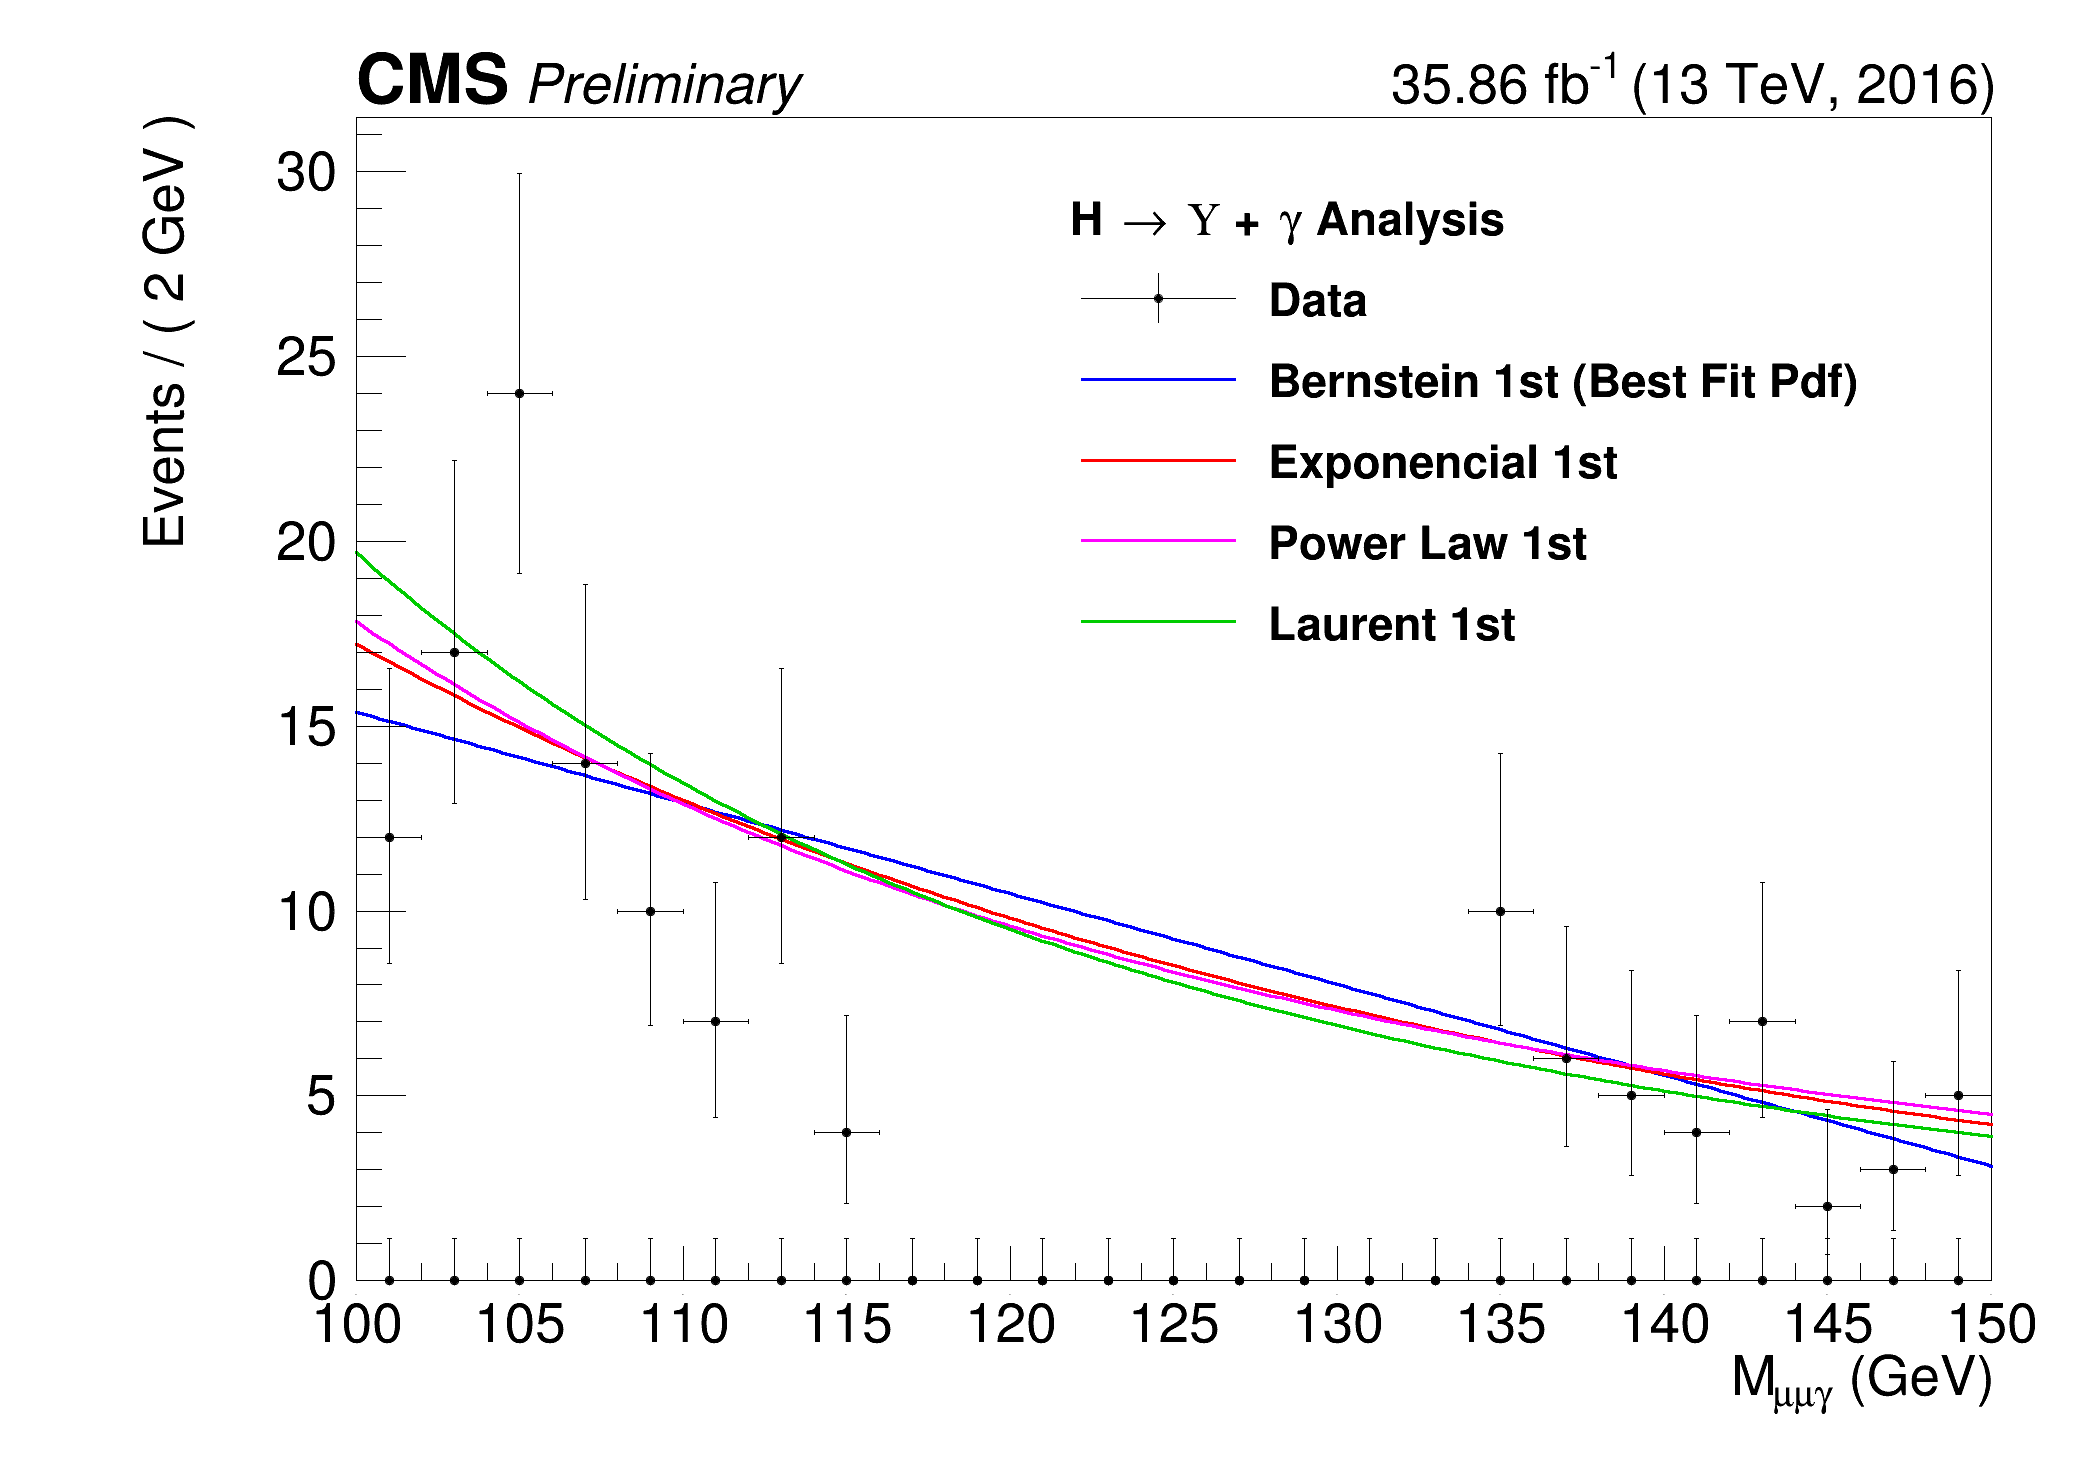
\includegraphics[width=0.45\textwidth]{figures_and_tables/fitPlotFiles2D/ftestOutput2D/outdir_HToUpsilonPhoton_Cat0/bkgfTest-Data/mHZ_multipdf_UntaggedTag_0}\hspace*{1.cm}
\end{center}\vspace*{-.5cm}
\caption{$H \rightarrow \Upsilon(1S,2S,3S) +\gamma$ Background Modeling: $\mu\mu\gamma$ distribution. The plotted \textit{pdfs} corresponds to the best choice by the statistical test for each family. The signal region, from 115 GeV to 135 GeV was blinded.}
\label{fig:HToUpsilon_mHZ_Projection}
\end{figure}


